\documentclass[]{beamer}
\usepackage[T1]{fontenc}
\usepackage[utf8]{inputenc}
\usepackage{lmodern}
\usepackage[italian]{babel}
\usepackage{cancel}
\usepackage{mathrsfs}

\title{Il magnetismo}
\author{\texorpdfstring{Mattia Cozzi\newline\href{mailto:cozzimattia@gmail.com}{\texttt{cozzimattia@gmail.com}}}{Mattia Cozzi}}
\date{a.s.~2023/2024}

%\documentclass[handout]{beamer}     %usare questa classe per generare l'handout
%\usepackage{pgfpages}   %per mostrare più quadri nella stessa pagina
%\pgfpagesuselayout{4 on 1}[a4paper,border shrink=5mm,landscape]
\usetheme{Singapore}
%\useoutertheme[left]{sidebar} %elementi intorno alle diapositive
\setbeamercovered{dynamic} %modifica l'aspetto del testo grigetto delle diapositive future. Argomenti: invisible/transparent/dynamic
\usecolortheme{orchid}
%COLORE PRINCIPALE
% \definecolor{marroncino}{RGB}{156, 26, 0} % UBC Blue (primary)
% \setbeamercolor{structure}{fg=marroncino} % itemize, enumerate, etc


\theoremstyle{plain}
\newtheorem{teorema}{Teorema}

\usepackage{tikz}


\usepackage{pgf,pgfplots,graphicx}
\usetikzlibrary{angles,quotes,arrows,shapes,decorations.markings}
\pgfplotsset{compat=1.15}
\usepgfplotslibrary{units,fillbetween} % to add units easily to axis
\tikzset{fleche/.style args={#1:#2}{postaction=decorate,decoration={name=markings,mark=at position #1 with {\arrow[#2,scale=2]{>}}},},}



\begin{document}

\begin{frame}
  \titlepage
\end{frame}





\begin{frame}
\frametitle{Contenuti}
\tableofcontents
\end{frame}

\section{Magnetismo}

\begin{frame}
\frametitle{Fenomeni magnetici fondamentali}
\begin{columns}
\begin{column}{0.3\textwidth}
\begin{figure}
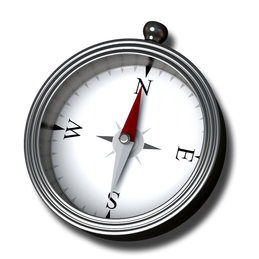
\includegraphics[width=\columnwidth]{img/bussola.png}
\end{figure}
Il magnetismo terrestre permette di orientarsi\\~
\end{column}
\begin{column}{0.3\textwidth}
\visible<2-3>{\begin{figure}
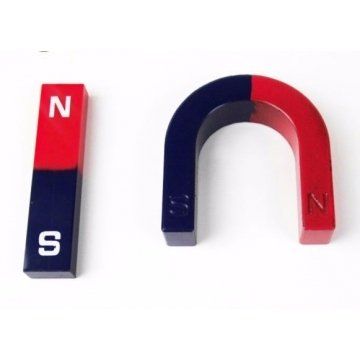
\includegraphics[width=\columnwidth]{img/calamite.jpg}
\end{figure}
I poli delle calamite si possono attrarre o respingere\\~}
\end{column}
\begin{column}{0.3\textwidth}
\visible<3>{\begin{figure}
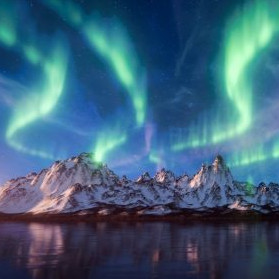
\includegraphics[width=\columnwidth]{img/aurora.jpg}
\end{figure}
L'aurora boreale è conseguenza del magnetismo terrestre}
\end{column}
\end{columns}
\end{frame}

\begin{frame}
\frametitle{Magneti}
\begin{columns}
\begin{column}{0.4\textwidth}
\begin{figure}
\textbf{Magneti naturali}\\~\\~
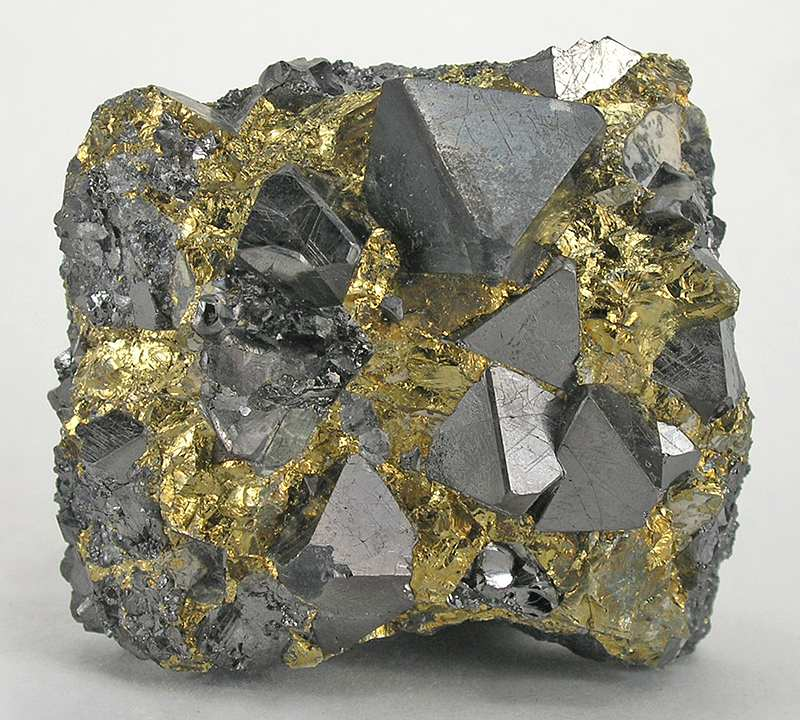
\includegraphics[width=\columnwidth]{img/magnetite.jpg}
Magnetite
\end{figure}
\end{column}
\begin{column}{0.4\textwidth}
\visible<2->{\begin{figure}
\textbf{Magneti artificiali}\\~\\~
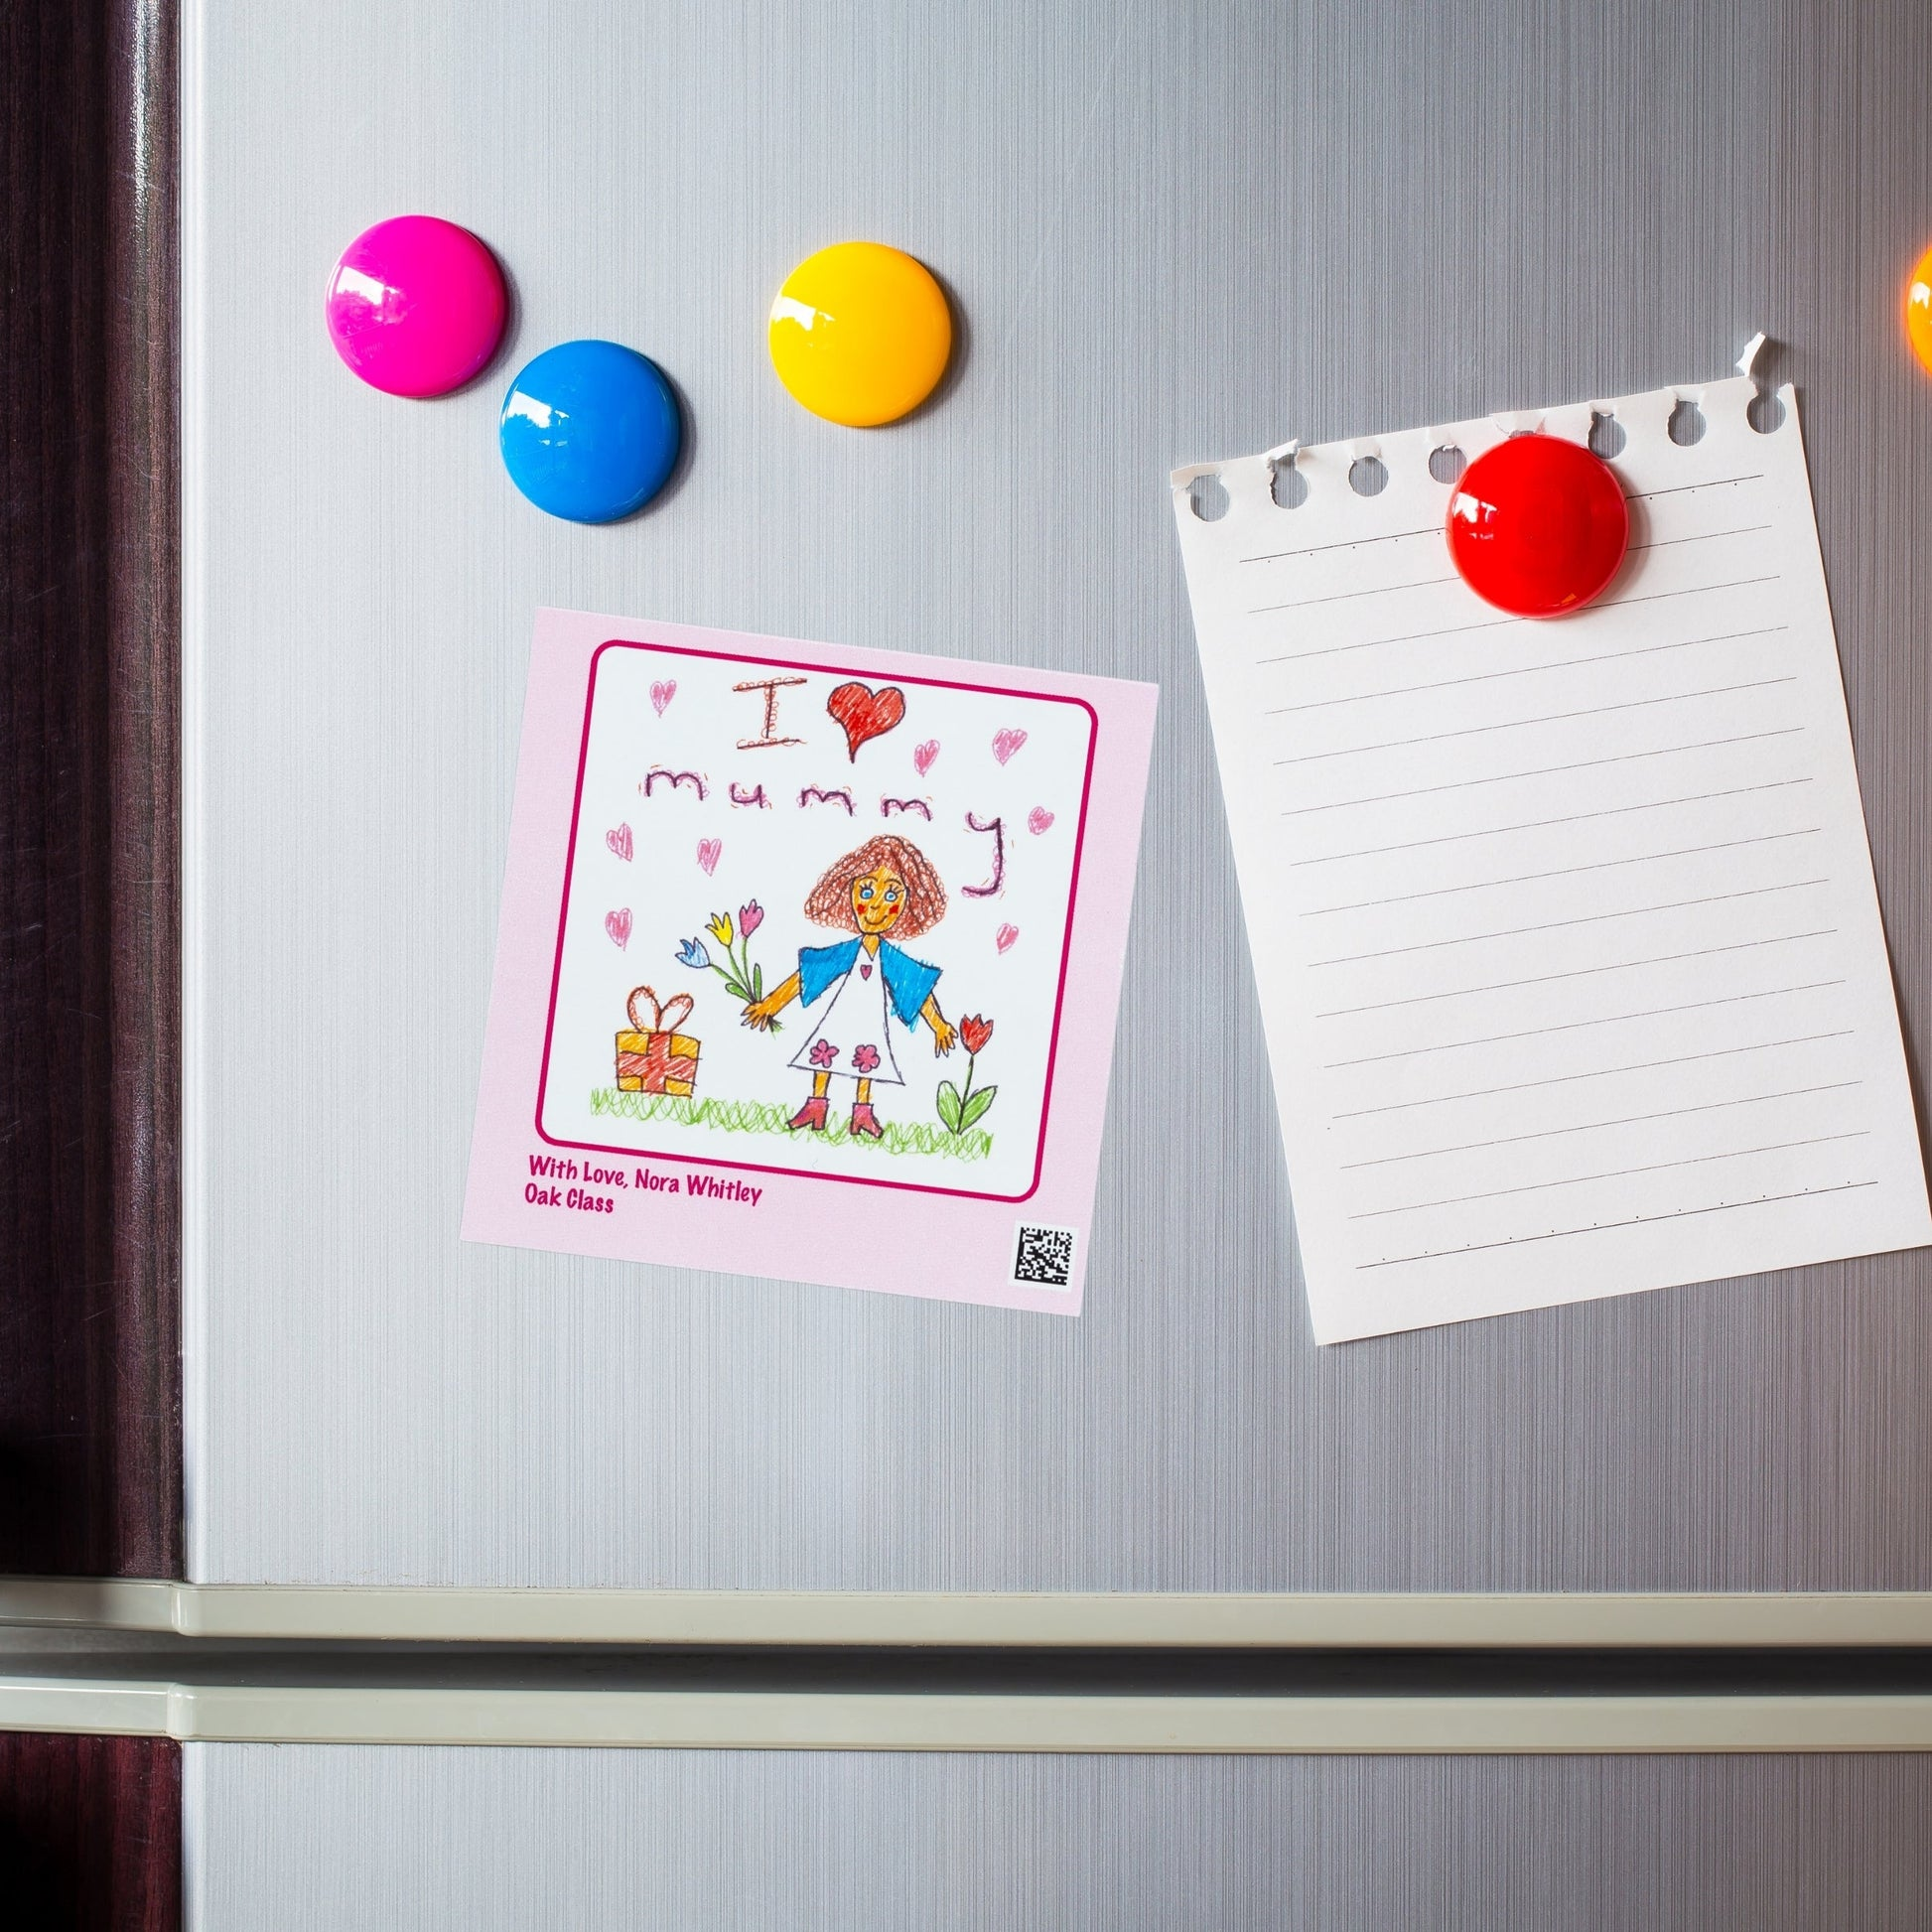
\includegraphics[width=\columnwidth]{img/frigo.jpg}
Calamite
\end{figure}}
\end{column}
\end{columns}
\end{frame}

\begin{frame}
\frametitle{Sostanze ferromagnetiche}
\begin{block}{Definizione}
I materiali che possono essere magnetizzati sono detti \emph{sostanze ferromagnetiche.}
\end{block}\pause

~

Sono ferromagnetici ferro, nichel, cobalto, neodimio e le loro leghe (ad esempio l'acciaio).
\end{frame}



\begin{frame}
\frametitle{Definizione operativa dei poli magnetici}
Una calamita (come l'ago di una bussola) libera di muoversi orienta sempre una sua parte verso un punto in prossimità del polo nord geografico terrestre.\pause

~

Definiamo tale parte della calamita \alert{polo nord} del magnete, l'altro sarà il \alert{polo sud}.
\end{frame}


\begin{frame}
\frametitle{Caratteristiche dei poli magnetici}
Possiamo verificare sperimentalmente che:
\begin{itemize}
  \item \alert<1>{poli dello stesso tipo si respingono}, poli di tipo diverso si attraggono;\pause
  \item i poli magnetici sono \alert{indivisibili}: rompendo una calamita in due parti, si ottengono due calamite!
\end{itemize}
\visible<2->{\begin{figure}
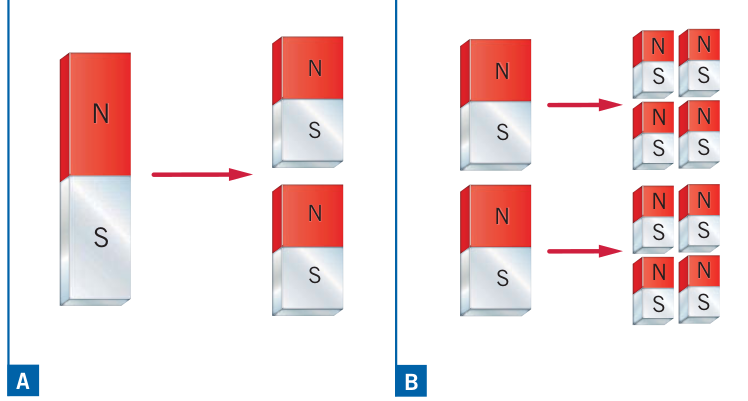
\includegraphics[width=.6\columnwidth]{img/divisionecalamite.png}
\end{figure}}
\end{frame}


\begin{frame}
\frametitle{Campo magnetico}
I magneti interagiscono tra loro generando nello spazio circostante un \alert<1>{campo magnetico}.\pause

~

Il \alert<2>{vettore campo magnetico} si indica con $ \vec{B} $ e si misura in \emph{tesla} $ [T] $.\pause

~

Il \alert<3>{verso positivo del vettore campo magnetico} sarà definito dal polo nord del \emph{magnete di prova}.
\visible<3->{\begin{figure}
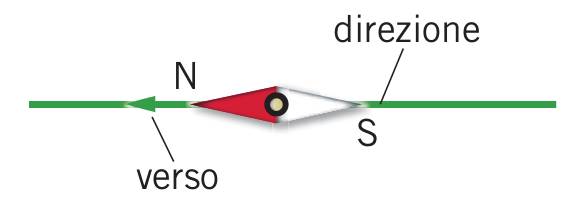
\includegraphics[width=.4\columnwidth]{img/magnetediprova.png}
\end{figure}}
\end{frame}



\begin{frame}
\frametitle{Linee di campo}
Possiamo visualizzare un campo magnetico con le linee di campo, che risultano \alert<1>{uscenti dal polo nord} ed entranti nel polo sud.

~

\begin{figure}
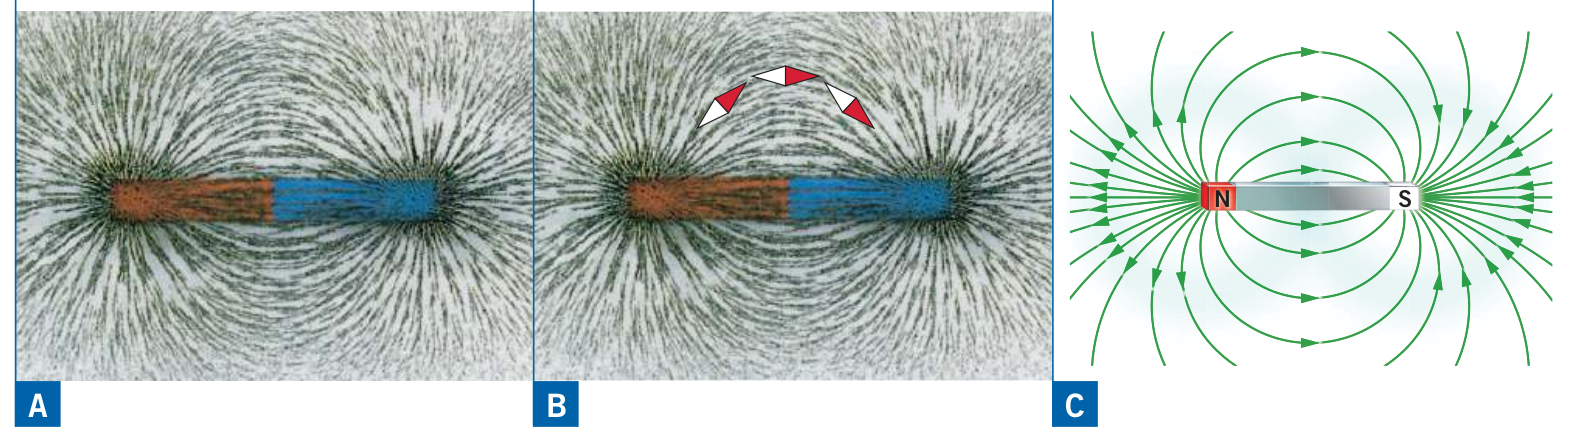
\includegraphics[width=\columnwidth]{img/lineemagnetico.png}
\end{figure}\pause
\alert{$ \vec{B} $ sarà in ogni punto tangente alle linee di campo} e direttamente proporzionale alla loro densità.
\end{frame}


\begin{frame}
\frametitle{Il campo magnetico terrestre}
\begin{figure}
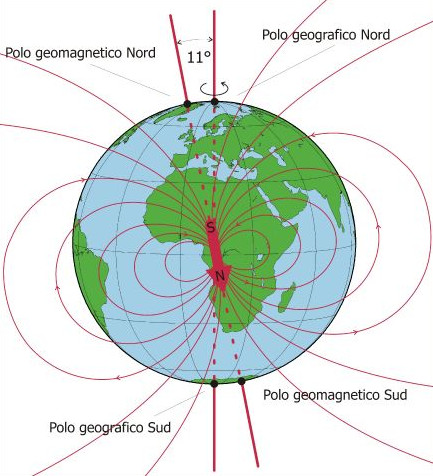
\includegraphics[width=.5\columnwidth]{img/campoterrestre.jpg}
\end{figure}
\end{frame}



\begin{frame}
\frametitle{Confronto con il campo elettrico}
\begin{columns}
\begin{column}{0.5\textwidth}
\begin{figure}
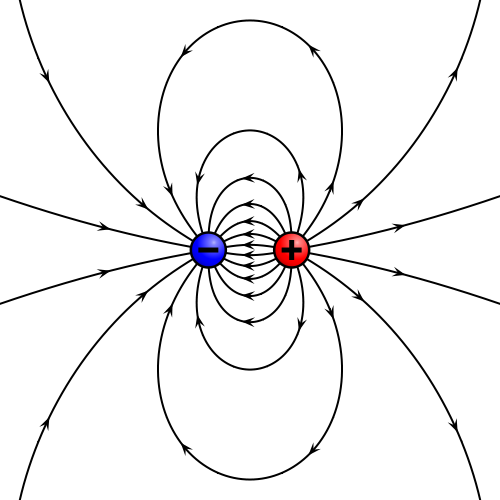
\includegraphics[width=.5\columnwidth]{img/dipoloelettrico.png}
\end{figure}
\visible<2->{Analogie:}
\begin{itemize}
  \item<2-> \alert<2>{sono campi di forza};
  \item<3-> \alert<3>{sono descritti da linee di campo};
  \item<4-> \alert<4>{ci sono due tipi di carica e due poli magnetici};
  \item<5-> \alert<5>{avvengono fenomeni di repulsione e attrazione}.
\end{itemize}
\end{column}
\begin{column}{0.5\textwidth}
\begin{figure}
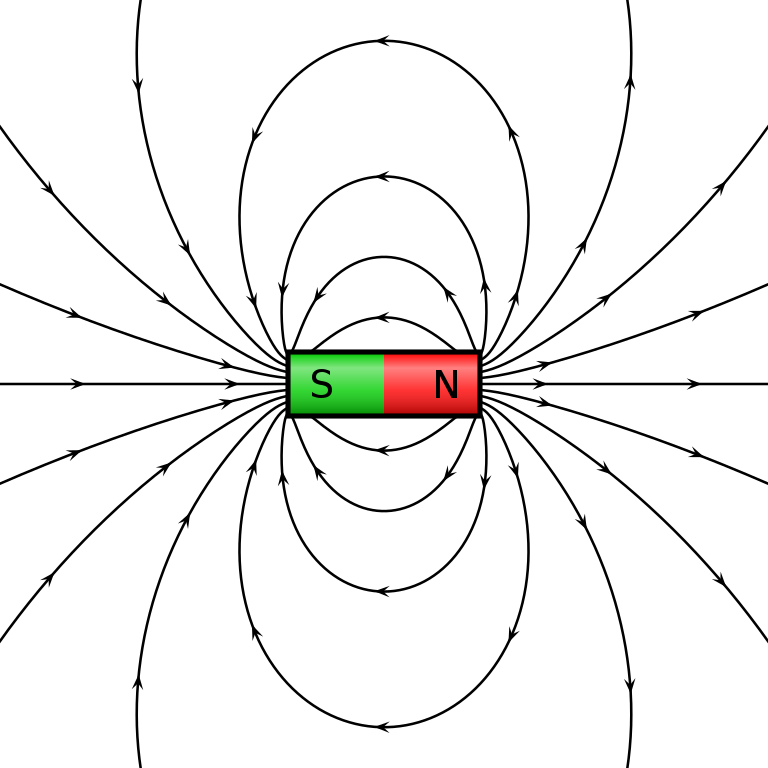
\includegraphics[width=.5\columnwidth]{img/dipolomagnetico.png}
\end{figure}
\visible<6->{Differenze:}
\begin{itemize}
  \item<6-> \alert<6>{le cariche si spostano tra corpi, i poli no};
  \item<7-> \alert<7>{esistono monopoli e dipoli elettrici, ma solo dipoli magnetici};
  \item<8-> \alert<8>{le linee del c.m.~sono sempre chiuse}.
\end{itemize}
\end{column}
\end{columns}
\end{frame}

\section{Interazione}

\begin{frame}
\frametitle{L'esperimento di {\O}rsted (1820)}
Il fisico danese Hans {\O}rsted si accorse che l'ago di una bussola, posto in prossimità di un filo percorso da corrente, \alert<1>{si orienta sempre perpendicolarmente al filo}.\pause

\visible<2->{\begin{figure}
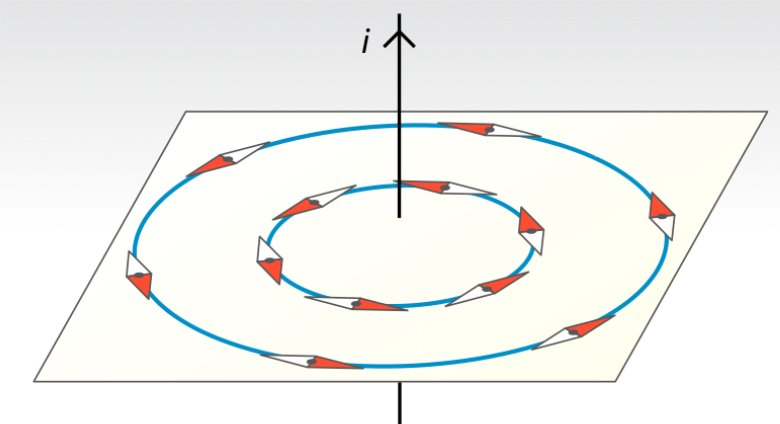
\includegraphics[width=.5\columnwidth]{img/oersted1.jpg}
\end{figure}}\pause
 
Per la prima volta ci si accorse di una \alert{interazione tra fenomeni elettrici e magnetici}.
\end{frame}


\begin{frame}
\frametitle{Campo magnetico di un filo percorso da corrente}
\begin{figure}
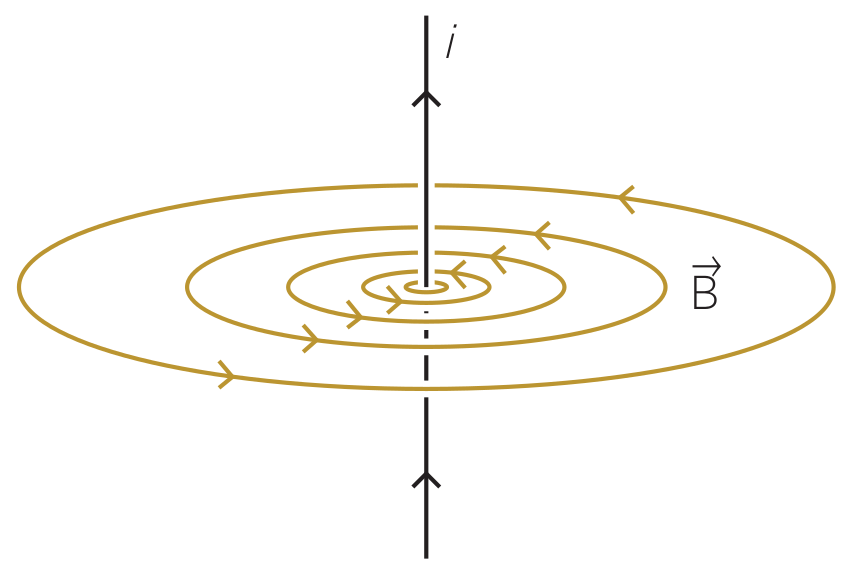
\includegraphics[width=.5\columnwidth]{img/oersted2.png}
\end{figure}
Il campo magnetico generato dal filo:
\begin{itemize}
  \item ha \alert<1>{linee circolari} con centro nel filo che giacciono su piani perpendicolari al filo;\pause
  \item è, in ogni punto dello spazio, \alert<2>{tangente a tali linee};\pause
  \item \alert<3>{diminuisce allontanandosi} dal filo.
\end{itemize}
\end{frame}



\begin{frame}
\frametitle{Verso di rotazione del campo magnetico}
\begin{figure}
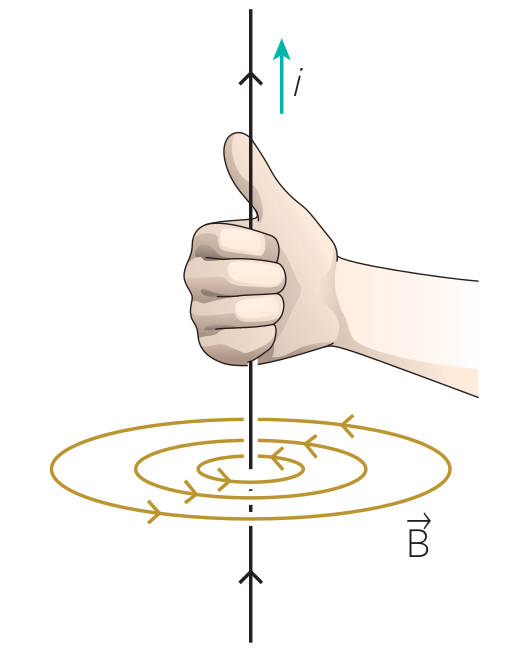
\includegraphics[width=.5\columnwidth]{img/oersted3.png}
\end{figure}
\end{frame}




\begin{frame}
\frametitle{L'esperimento di Faraday (1821)}
\begin{columns}
\begin{column}{0.45\textwidth}
Come possiamo \emph<1>{misurare} l'intensità di $ \vec{B} $?\pause

~

Michael Faraday scopre nel 1821 che un filo percorso da corrente \alert<2>{subisce una forza se immerso in un campo magnetico}.\pause
\end{column}
\begin{column}{0.5\textwidth}
\visible<3>{\begin{figure}
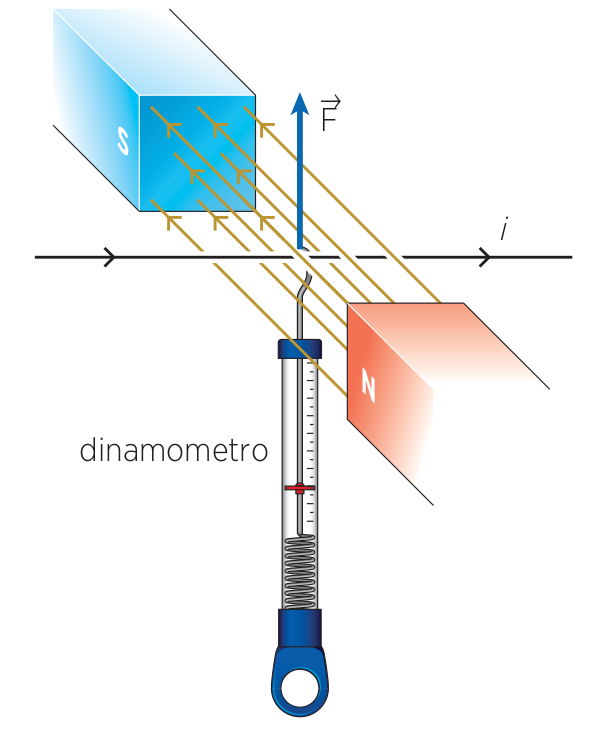
\includegraphics[width=\columnwidth]{img/espfaraday1.png}
\end{figure}}
\end{column}
\end{columns}
\end{frame}



\begin{frame}
\frametitle{Intensità del campo magnetico}
Si vede sperimentalmente che:
\begin{columns}
\begin{column}{0.3\textwidth}
\begin{itemize}
  \item $ F \propto B $;
\end{itemize}
\end{column}
\begin{column}{0.3\textwidth}
\begin{itemize}
  \item $ F \propto i $;
\end{itemize}
\end{column}
\begin{column}{0.3\textwidth}
\begin{itemize}
  \item $ F \propto \ell $.
\end{itemize}
\end{column}
\end{columns}\pause

~

~

Esprimiamo questi fatti definendo l'intensità di $ \vec{B} $ come:
\begin{center}
~~~~~~~~~~~~~~~~~~~~~\colorbox{blue!30}{$ B = \dfrac{F}{i\ell} $}\pause~~~~~~~~~$ \left[ T \right] = \left[ \dfrac{N}{A\cdot m} \right] $
\end{center}\pause

~

In particolare, \alert<4>{se il filo e il campo sono perpendicolari la forza è massima e vale:}
\begin{center}
\colorbox{blue!30}{$ F=Bi\ell $}
\end{center}
\end{frame}

\begin{frame}
\frametitle{Esempi}
\begin{columns}
\begin{column}{0.4\textwidth}
\begin{figure}
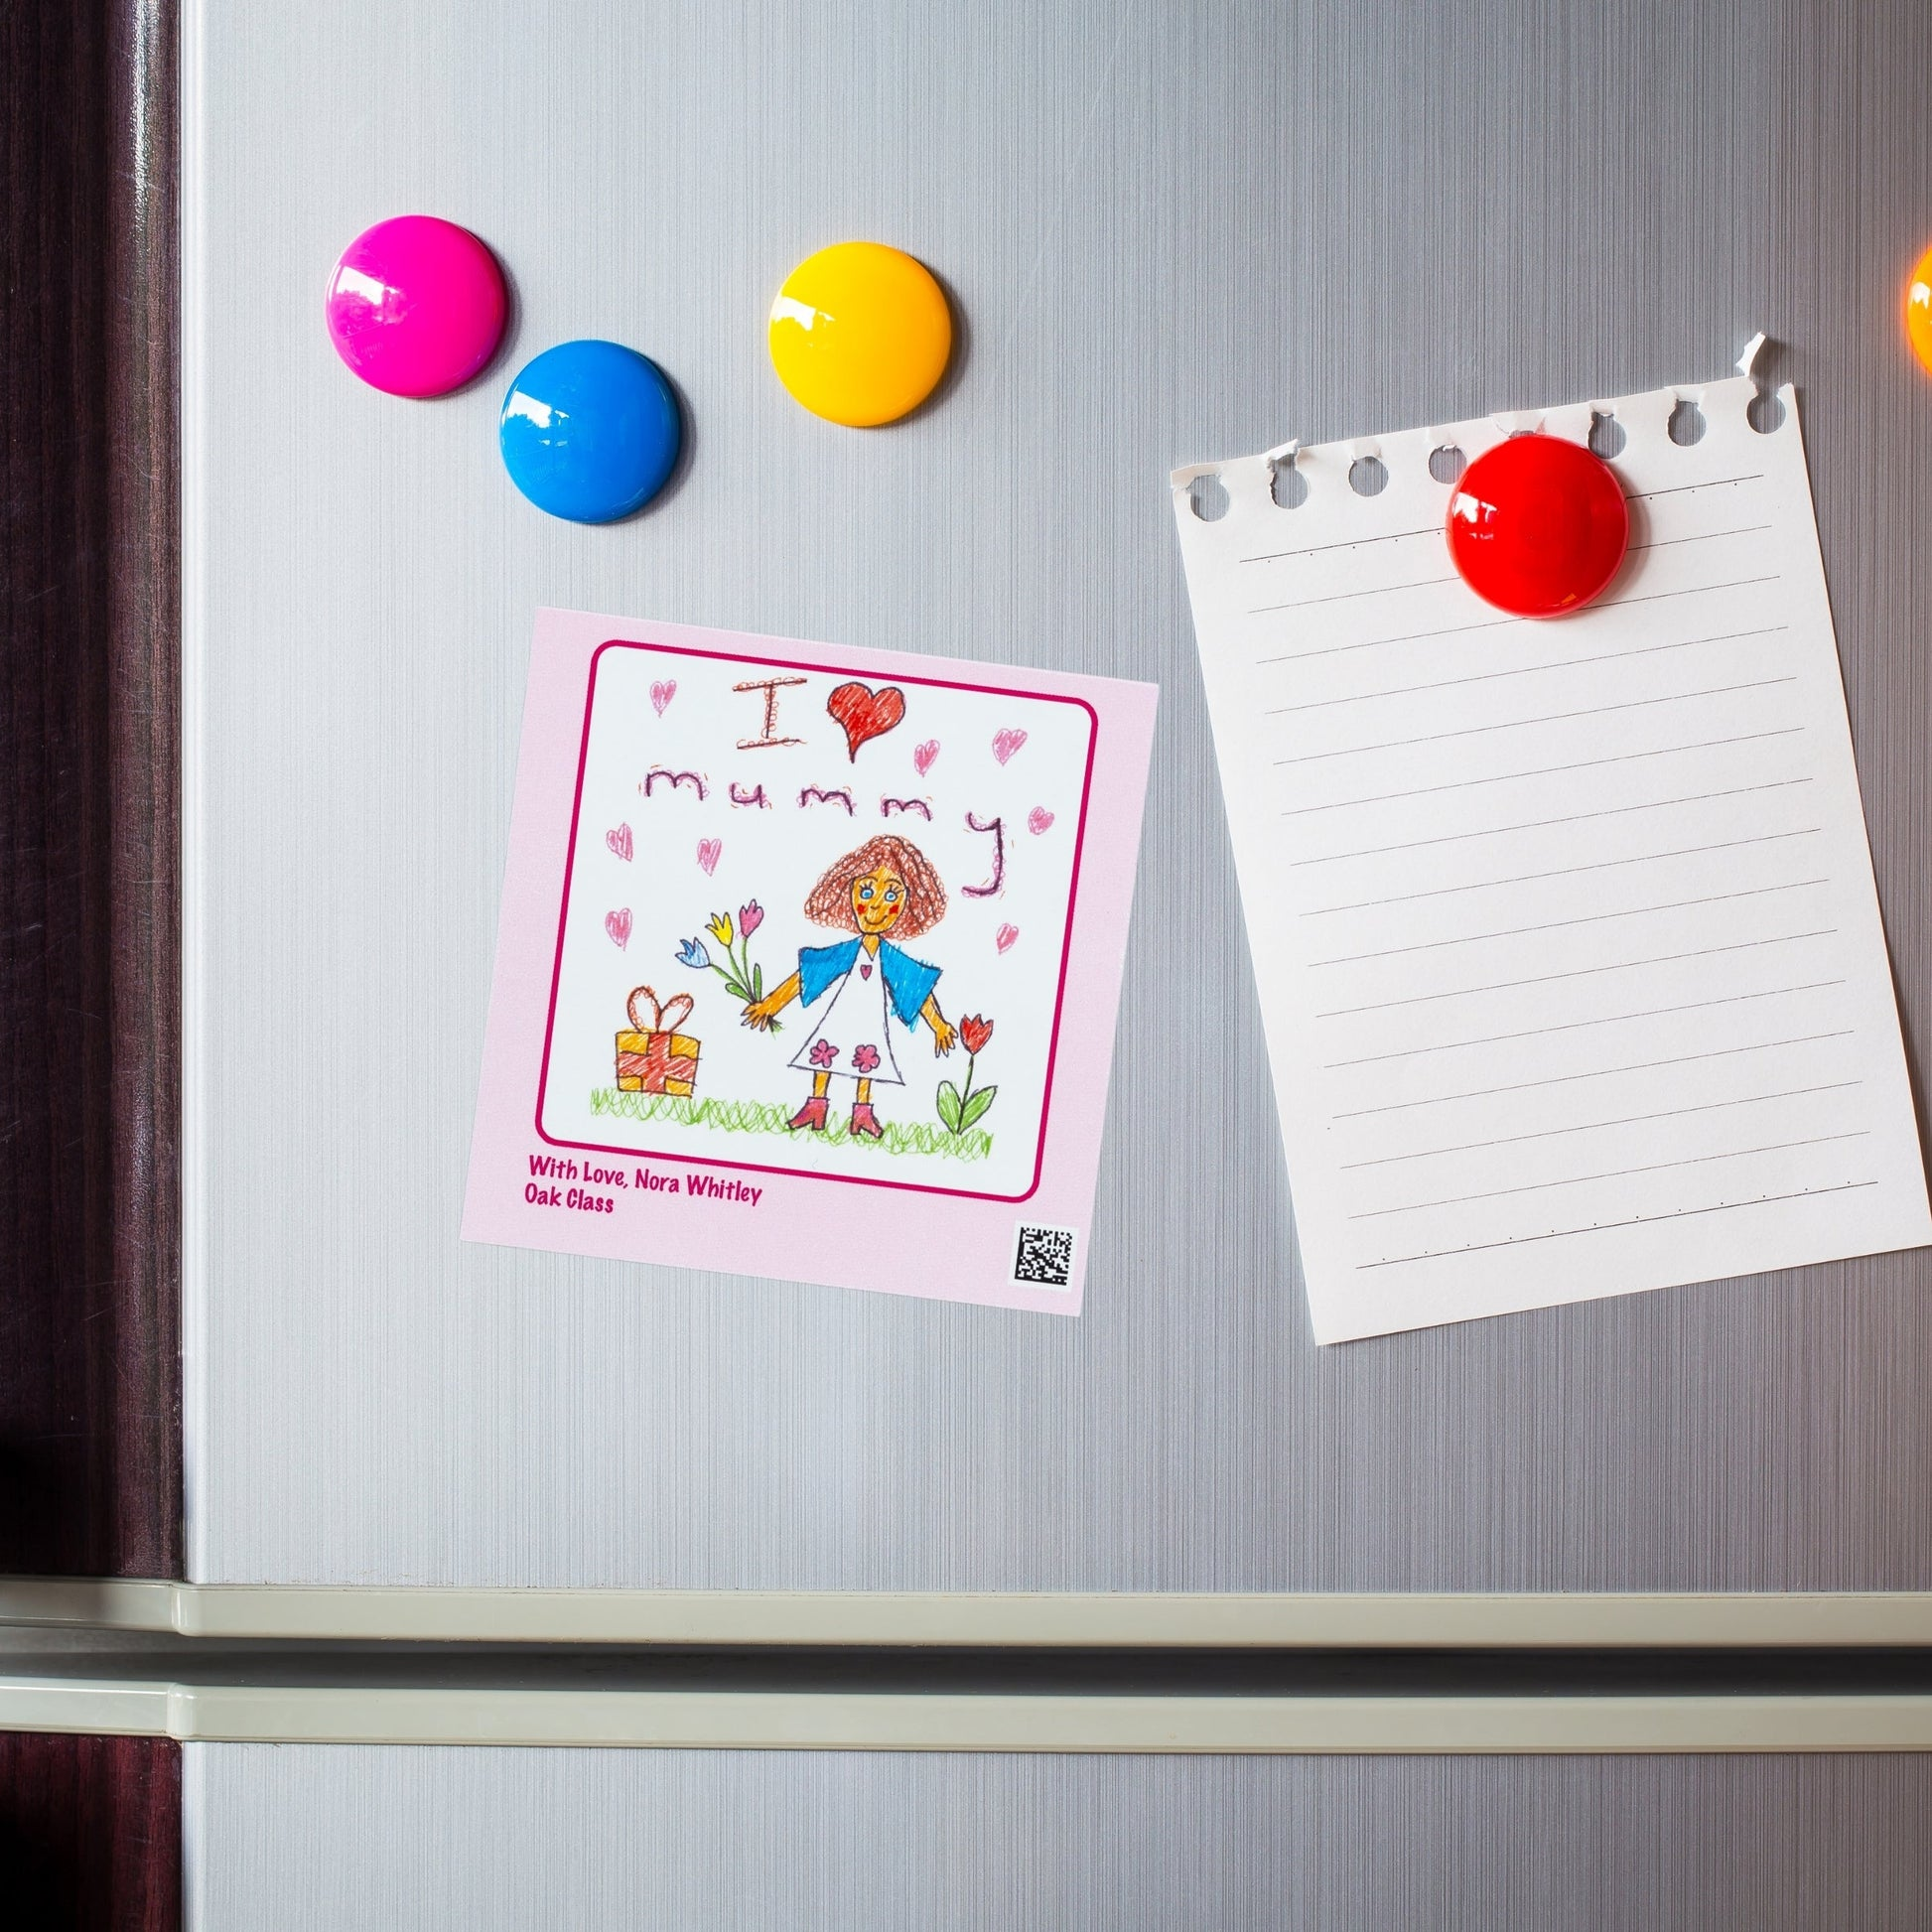
\includegraphics[width=\columnwidth]{img/frigo.jpg}
$ 6 \, mT $
\end{figure}
\end{column}
\begin{column}{0.4\textwidth}
\visible<2->{\begin{figure}
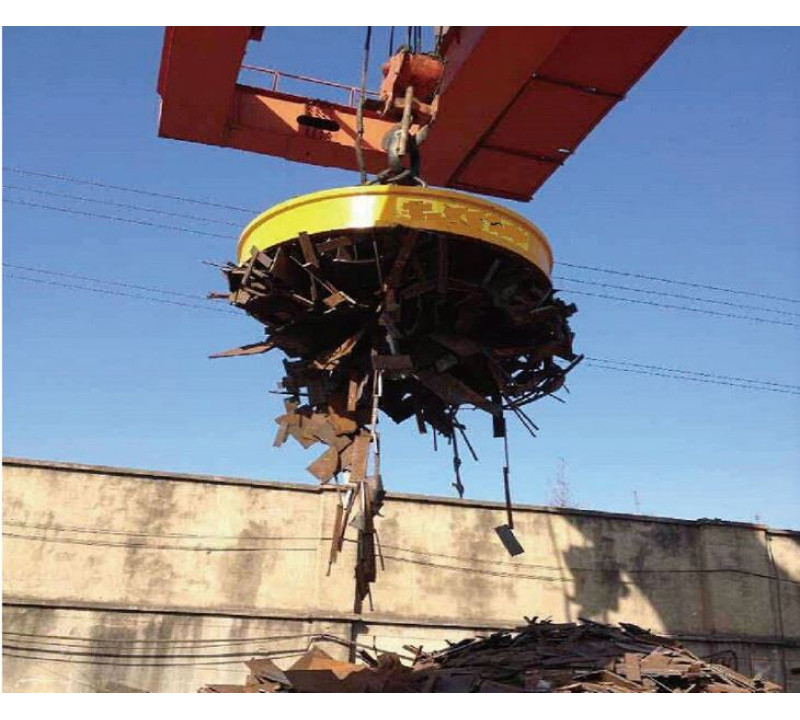
\includegraphics[width=\columnwidth]{img/rottami.jpg}
$ 2 \, T $
\end{figure}}
\end{column}
\end{columns}
\end{frame}



\begin{frame}
\frametitle{Direzione e verso della forza magnetica}
\begin{figure}
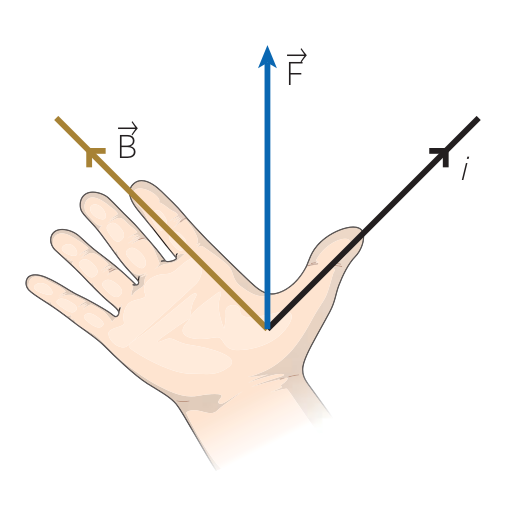
\includegraphics[width=.5\columnwidth]{img/espfaraday2.png}
\end{figure}
\end{frame}



\begin{frame}
\frametitle{Esercizio}
\begin{exampleblock}{Intensità del campo magnetico}
  Un filo lungo $ 50 \, cm $, percorso da una corrente di $ 7,23 \times 10^{-3} \, A $, è immerso in un campo magnetico uniforme di intensità $ B $ e si trova nella posizione per cui la forza che agisce su di esso è massima e pari a $ 3,2 \, N $.

  ~

  Quanto vale $ B $?\hspace{\fill}[$ 8,9 \times 10^{2} \, T $]
\end{exampleblock} 
\end{frame}


\begin{frame}
\frametitle{Caso generale}
Sappiamo che:
\begin{itemize}
  \item $ \vec{F} $ è \alert<1>{perpendicolare al piano individuato dal filo e dal campo};\pause
  \item la forza è massima con filo e campo perpendicolari: \alert<2>{dipende dalla componente di $ \vec{B} $ perpendicolare al filo}.
\end{itemize}\pause

~

\begin{columns}
\begin{column}{0.5\textwidth}
Possiamo pertanto ricorrere al \alert<3>{prodotto vettoriale}:
\begin{center}
\colorbox{blue!30}{$ \vec{F}=i \vec{\ell}\times \vec{B} $}

~

$ F = i\ell B\sin\alpha $
\end{center}
\end{column}
\begin{column}{0.4\textwidth}
\visible<3->{\begin{figure}
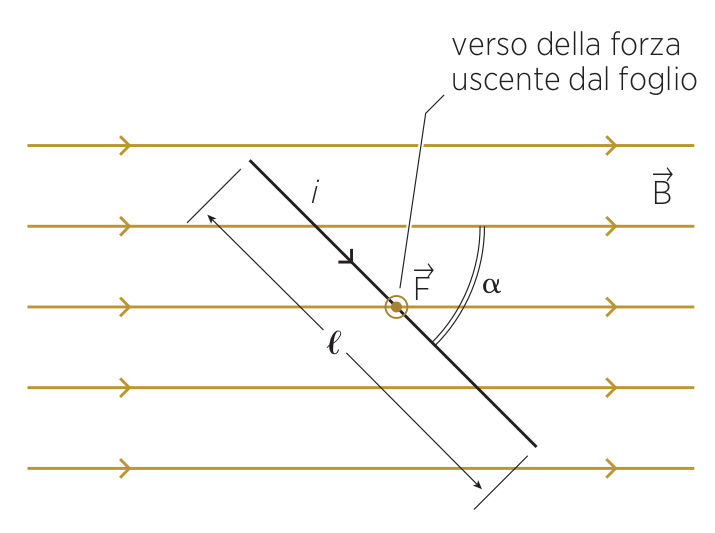
\includegraphics[width=\columnwidth]{img/forzafilo.png}
\end{figure}}
\end{column}
\end{columns}
\end{frame}


\begin{frame}
\frametitle{Esercizio}
\begin{exampleblock}{Calcolo dell'angolo}
  Un tratto di conduttore rettilineo lungo $ 20,0 \, cm $ è posto tra le espansioni di un magnete. Il campo magnetico è uniforme e la sua intensità vale $ 0,400 \, T $. Quando nel conduttore circola una corrente elettrica continua di $ 0,320 \, A $, si misura una forza magnetica che agisce sul conduttore e si trova che $ F = 1,28 \times 10^{-2} \, N $.

  ~

  Determina l'angolo formato dal conduttore con il campo magnetico.\hspace{\fill}[$ 30^\circ \vee 150^\circ $]
\end{exampleblock} 
\end{frame}


\begin{frame}
\frametitle{L'esperimento di Ampère (un settimana dopo \O rsted)}
\begin{columns}
\begin{column}{0.4\textwidth}
Sappiamo:
\begin{itemize}
  \item da \O rsted, che \alert<1>{una corrente genera un campo magnetico};\pause
  \item da Faraday, che \alert<2>{una corrente subisce una forza magnetica}.\pause
\end{itemize}

~

Conclusione: \alert<3>{due fili percorsi da corrente eserciteranno una forza l'uno sull'altro}.
\end{column}
\begin{column}{0.5\textwidth}
\visible<3->{\begin{figure}
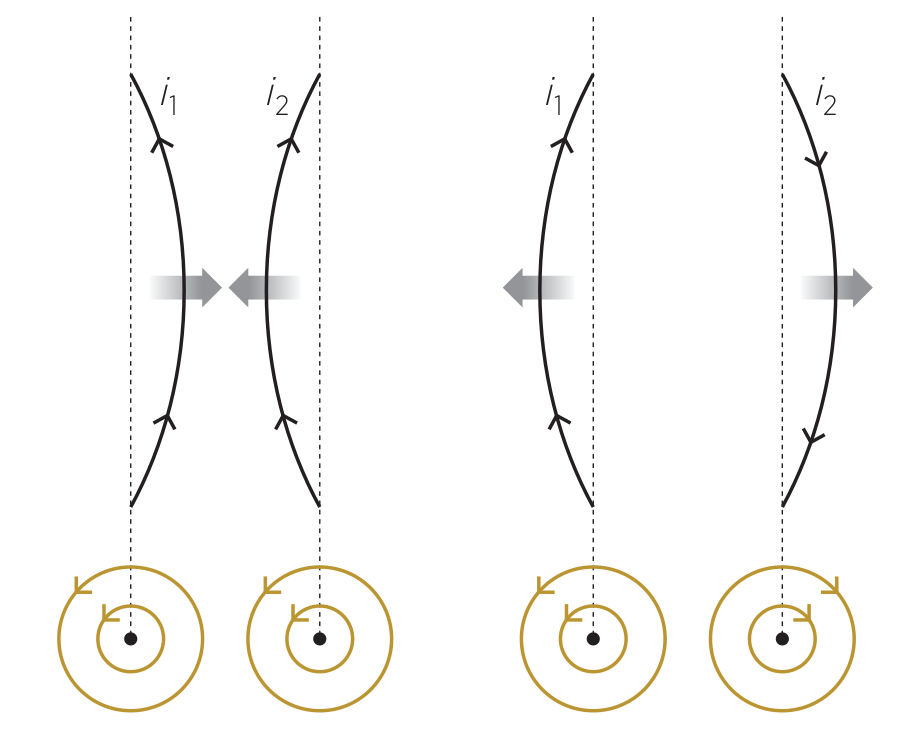
\includegraphics[width=\columnwidth]{img/espampere.png}
\end{figure}}
\end{column}
\end{columns}
\end{frame}

\begin{frame}
\frametitle{Legge di Ampère}
Si verifica sperimentalmente che:
\begin{columns}
\begin{column}{0.3\textwidth}
\begin{itemize}
  \item $ F \propto i_1, i_2 $;
\end{itemize}
\end{column}
\begin{column}{0.3\textwidth}
\begin{itemize}
  \item $ F \propto \ell $;
\end{itemize}
\end{column}
\begin{column}{0.3\textwidth}
\begin{itemize}
  \item $ F \propto \dfrac{1}{d} $.
\end{itemize}
\end{column}
\end{columns}\pause

~

~

Otteniamo pertanto la legge:
\begin{center}
\colorbox{blue!30}{$ F = \dfrac{\mu_0}{2\pi} \cdot \dfrac{i_1i_2}{d}\ell $}
\end{center}
con:
\begin{center}
\colorbox{blue!30}{$ \mu_0 = $ permeabilità magnetica del vuoto $ = 4\pi \times 10^{-7} \, \dfrac{N}{A^2} $}
\end{center}
\end{frame}



\begin{frame}
\frametitle{Esercizio}
\begin{exampleblock}{Forza magnetica}
  In due lunghi fili conduttori rettilinei, che distano tra loro $ 2,2 \, cm $, sono presenti due correnti di intensità $ 3,8 \, A $ e $ 7,5 \, A $.

  ~

  Qual è il valore della forza magnetica che agisce su un tratto di filo lungo $ 2,0 \, m $?\hspace{\fill}[$ 5,2 \times 10^{-4} \, N $]
\end{exampleblock} 
\end{frame}


\begin{frame}
\frametitle{Una legge per l'esperimento di \O rsted}
Usiamo le nostre conoscenze per calcolare l'intensità di $ \vec{B} $ a distanza $ d $ da un filo rettilineo percorso da una corrente $ i $.\pause

~

Questo causa una forza $ \vec{F} $ su un altro filo percorso da corrente $ i_1 $. 

~

\begin{columns}
\begin{column}{0.5\textwidth}
Valgono:
\begin{center}
$ F = Bi_1\ell $~~~~~~~~~~~$ F = \dfrac{\mu_0}{2\pi} \cdot \dfrac{ii_1}{d}\ell $\pause

~

~

$ B\cancel{i_1}\cancel{\ell} = \dfrac{\mu_0}{2\pi} \cdot \dfrac{i\cancel{i_1}}{d}\cancel{\ell} $\pause

~

~

$ B = \dfrac{\mu_0}{2\pi} \cdot \dfrac{i}{d} $
\end{center}
\end{column}
\begin{column}{0.3\textwidth}
\visible<1->{\begin{figure}
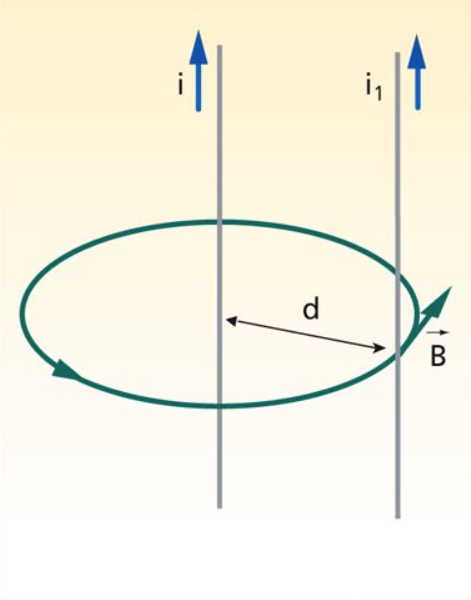
\includegraphics[width=\columnwidth]{img/leggeampere.png}
\end{figure}}
\end{column}
\end{columns}
\end{frame}






\begin{frame}
\frametitle{Legge di Biot-Savart}
\begin{figure}
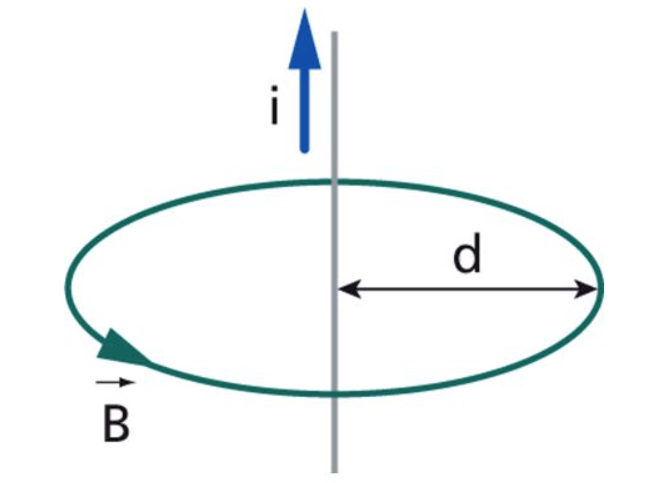
\includegraphics[width=.4\columnwidth]{img/biotsavart.png}
\end{figure}
Un filo percorso da corrente $ i $ genera a distanza $ d $ un campo magnetico di intensità:
\begin{center}
\colorbox{blue!30}{$ B = \dfrac{\mu_0}{2\pi} \cdot \dfrac{i}{d} = \mu_0 \cdot \dfrac{i}{2\pi d} $}
\end{center}
\end{frame}


\begin{frame}
\frametitle{Esercizio}
\begin{exampleblock}{Distanza dal filo}
  Alcuni pacemaker sono dotati di un interruttore magnetico che viene pilotato dall'esterno attraverso un campo magnetico. Per poter agire sul pacemaker, il campo deve avere un'intensità di $ 5 \times 10^{-4} \, T $. Tale campo viene generato tramite un filo percorso da corrente di intensità $ 1.2 \times 10^{3} \, A $ che è posizionato dal medico ad una distanza $ d $ dal paziente.

  ~

  Calcola il valore della distanza $ d $.\hspace{\fill}[$ 0,5 \, m $]
\end{exampleblock} 
\end{frame}


\section{Spire}



\begin{frame}
\frametitle{Spira percorsa da corrente}
Una spira è un filo conduttore di forma circolare.\pause

~


\begin{columns}
\begin{column}{0.5\textwidth}
Una spira di raggio $ R $ percorsa da una corrente $ i $ genera intorno a sé un campo magnetico.\pause

~

Il campo magnetico generato al centro della spira è rettilineo e vale:
\begin{center}
\colorbox{blue!30}{$ B = \dfrac{\mu_0}{2R} \cdot i $}
\end{center}
\end{column}
\begin{column}{0.4\textwidth}
\visible<2->{\begin{figure}
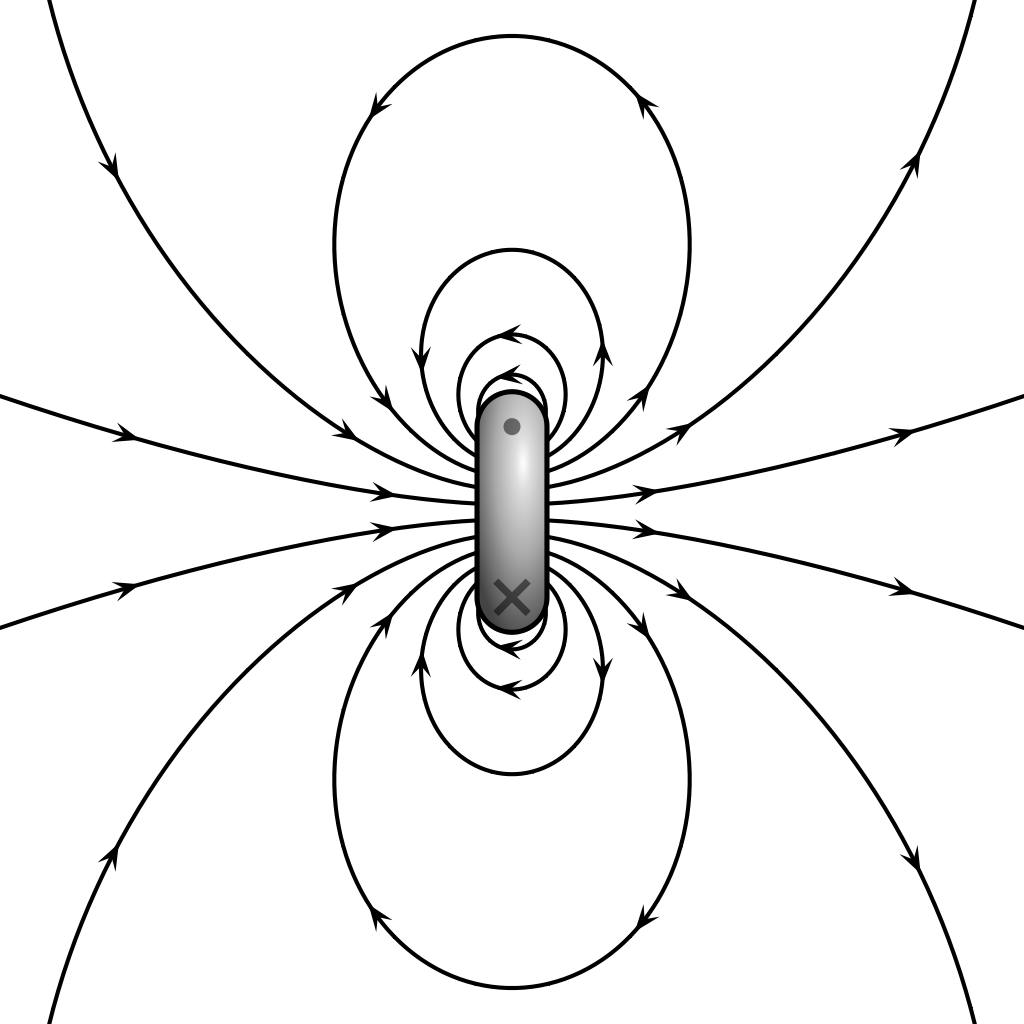
\includegraphics[width=\columnwidth]{img/spira.png}
\end{figure}}
\end{column}
\end{columns}
\end{frame}





\begin{frame}
\frametitle{Solenoide (1)}
\begin{columns}
\begin{column}{0.6\textwidth}
Un solenoide è un avvolgimento di filo conduttore (cioè una pila di spire).
\end{column}
\begin{column}{0.3\textwidth}
\visible<1->{\begin{figure}
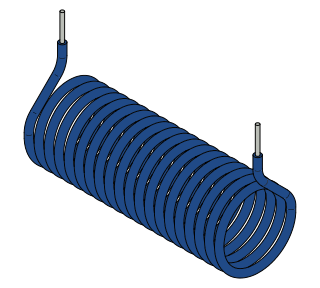
\includegraphics[width=.9\columnwidth]{img/solenoide.png}
\end{figure}}
\end{column}
\end{columns}\pause

~

Il campo di ogni spira viene sommato a quello delle altre:
\visible<2->{\begin{figure}
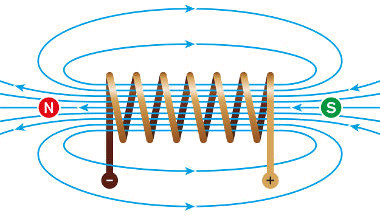
\includegraphics[width=.5\columnwidth]{img/solenoide.jpg}
\end{figure}}
\end{frame}





\begin{frame}
\frametitle{Solenoide (2)}
\begin{figure}
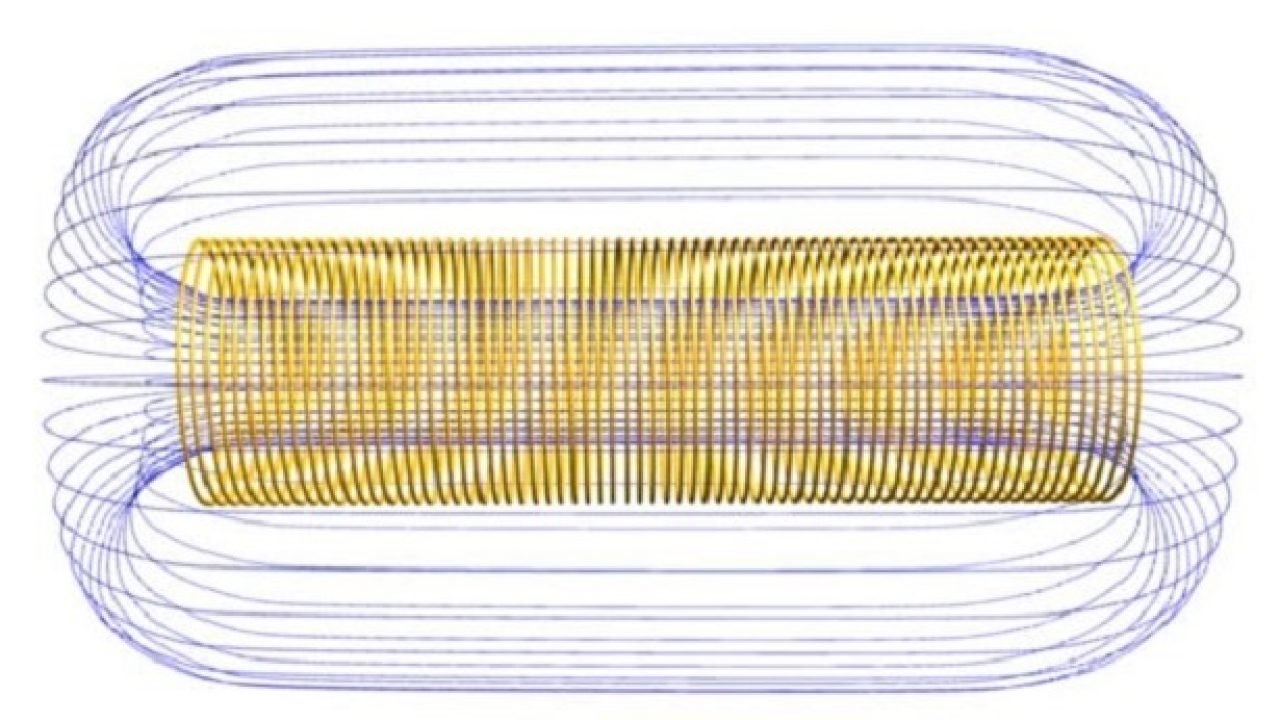
\includegraphics[width=.5\columnwidth]{img/solenoide2.jpg}
\end{figure}

Un solenoide percorso da corrente genera un campo al suo interno:
\begin{center}
\colorbox{blue!30}{$ B = \mu_0 \cdot \dfrac{Ni}{\ell} $}
\end{center}
\begin{columns}
\begin{column}{0.4\textwidth}
\begin{itemize}
  \item $ N= $ numero di spire
\end{itemize}
\end{column}
\begin{column}{0.5\textwidth}
\begin{itemize}
  \item $ \ell = $ lunghezza del solenoide
\end{itemize}
\end{column}
\end{columns}
\end{frame}


\section{Motore}


\begin{frame}
\frametitle{Cosa hanno in comune?}
\begin{columns}
\begin{column}{0.3\textwidth}
\begin{figure}
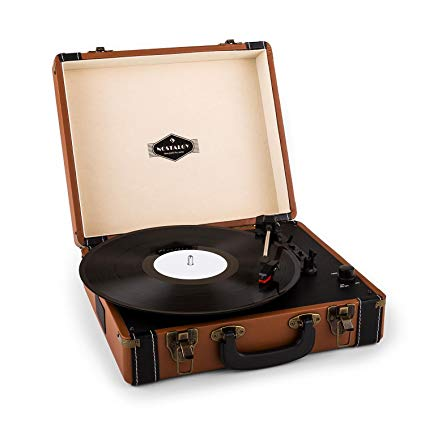
\includegraphics[width=\columnwidth]{img/giradischi.jpg}
\end{figure}
\end{column}
\begin{column}{0.3\textwidth}
\visible<2-3>{\begin{figure}
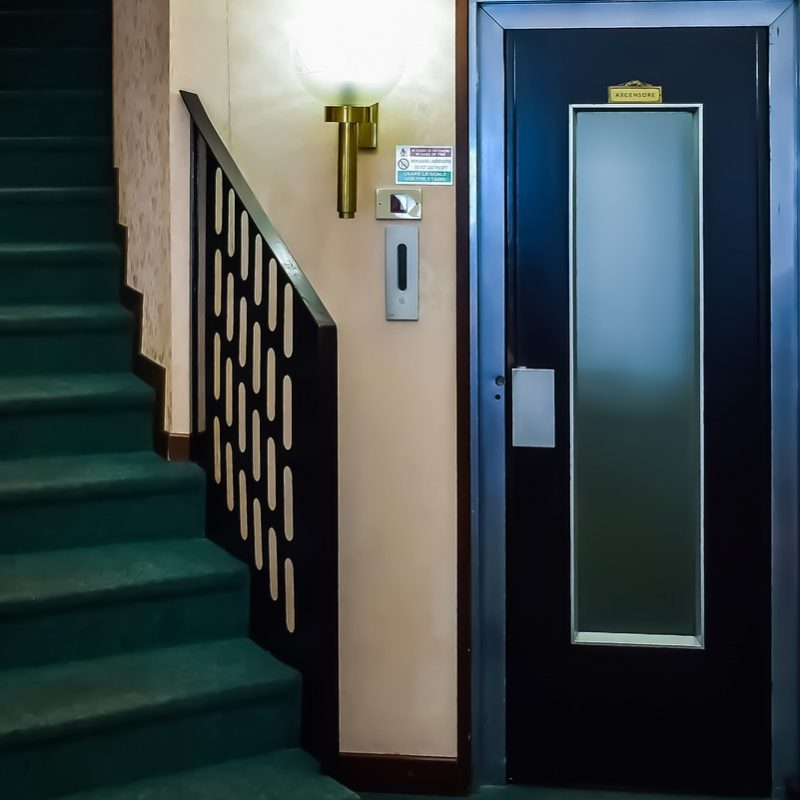
\includegraphics[width=\columnwidth]{img/ascensore.jpg}
\end{figure}}
\end{column}
\begin{column}{0.3\textwidth}
\visible<3>{\begin{figure}
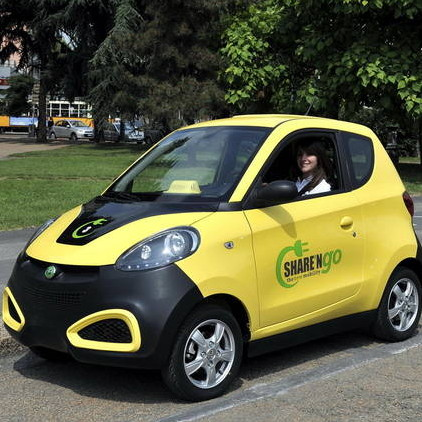
\includegraphics[width=\columnwidth]{img/autoelettrica.jpg}
\end{figure}}
\end{column}
\end{columns}
\end{frame}



\begin{frame}
\frametitle{Trasformazione di energia}
\begin{block}{Motore elettrico}
Un motore elettrico è un dispositivo che trasforma energia elettrica in energia meccanica.
\end{block}
\begin{columns}
\begin{column}{0.4\textwidth}
\visible<2->{\begin{figure}
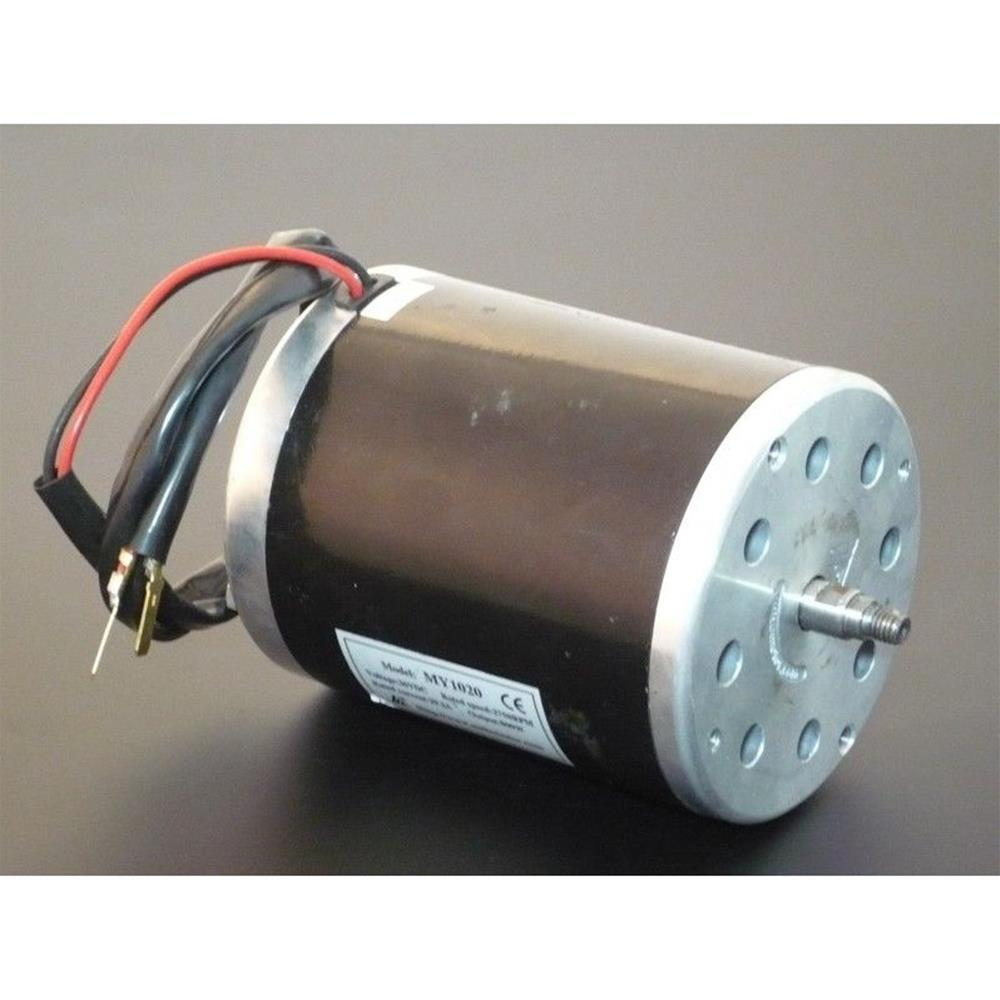
\includegraphics[width=\columnwidth]{img/motore1.jpg}
\end{figure}}
\end{column}
\begin{column}{0.4\textwidth}
\visible<3->{\begin{figure}
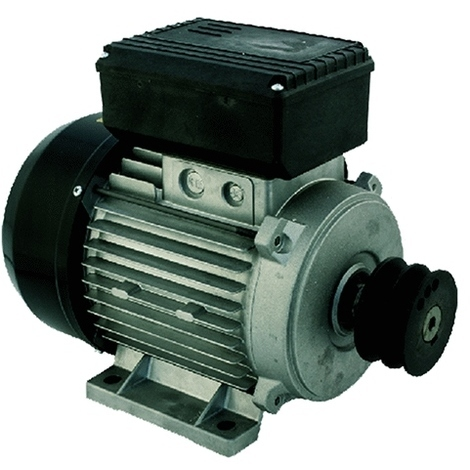
\includegraphics[width=\columnwidth]{img/motore2.jpg}
\end{figure}}
\end{column}
\end{columns}
\end{frame}

\begin{frame}
\frametitle{Modello di un motore elettrico}
\begin{figure}
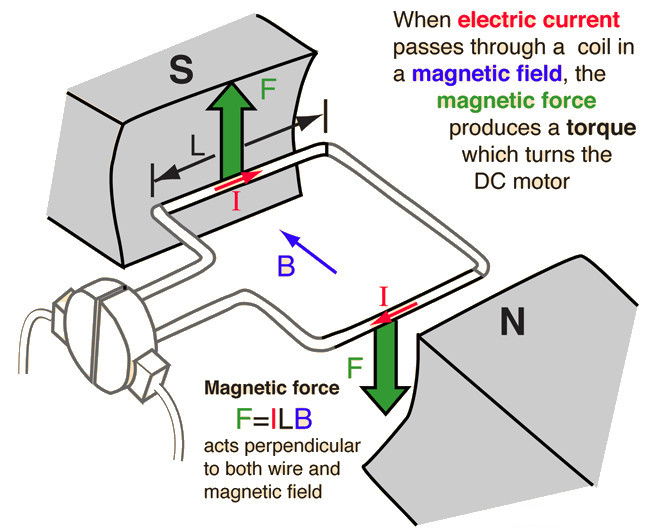
\includegraphics[width=.7\columnwidth]{img/schemamotore.jpg}
\end{figure}
\end{frame}


\begin{frame}
\frametitle{Modello di un motore elettrico (2)}
Il moto della spira dura finché essa non si dispone perpendicolarmente al campo.\pause

~

Le forze non tendono più a farla ruotare, ed è pertanto necessario invertire il verso della corrente, grazie ai \alert{commutatori ad anelli}.

~

\begin{center}
\href{video/Motoreelettrico.mp4}{\beamergotobutton{Video: Funzionamento di un motore elettrico}}
\end{center}
\begin{center}
\href{gif/motoreelettrico.gif}{\beamergotobutton{GIF: Funzionamento di un motore elettrico}}
\end{center}\pause
\begin{block}{Inversione della corrente}
Cambiando il verso della corrente ogni mezzo giro, la coppia di forze mantiene la spira in rotazione.
\end{block}
\end{frame}


\begin{frame}
\frametitle{Momento magnetico (1)}
Immaginiamo una spira rettangolare di dimensioni $ a $ e $ b $, percorsa da corrente $ i $, in un campo $ \vec{B} $ come in figura.

\begin{figure}
\begin{tikzpicture}[scale=.5]
\draw [thick] (0,0) -- (6,0)  -- (6,4) -- (0,4) -- (0,0);
\draw [->] (.3,1) -- (.3,3);
\draw [<-] (5.7,1) -- (5.7,3);
\node [right] at (.3,2) {{\tiny $ i $}};
\node [left] at (0,2) {{\tiny $ a $}};
\node [right] at (6,2) {{\tiny $ a $}};
\node [above] at (3,4) {{\tiny $ b $}};
\node [below] at (3,0) {{\tiny $ b $}};
\draw [<-,blue,thick] (1.5,2) -- (4.5,2);
\node [below,blue,thick] at (3,2) {{\tiny $ \vec{B} $}};
\draw [ultra thick,fill] (3,0) circle [radius=.05];
\node [above] at (3,0) {{\tiny $ O $}};
\end{tikzpicture}
\end{figure}\pause
Sappiamo che il momento della forza rispetto al punto $ O $ vale:
\begin{center}
$ M = forza \cdot braccio \cdot \sin\theta $
\end{center}
con $ \theta_{iniziale} = \dfrac{\pi}{2} $ e $ \theta_{finale} = \pi $ (spira perpendicolare al campo).
\end{frame}

\begin{frame}
\frametitle{Momento magnetico (2)}
\begin{columns}
\begin{column}{0.4\textwidth}
\begin{figure}
\begin{tikzpicture}[scale=.5]
\draw [thick] (0,0) -- (6,0)  -- (6,4) -- (0,4) -- (0,0);
\draw [->] (.3,1) -- (.3,3);
\draw [<-] (5.7,1) -- (5.7,3);
\node [right] at (.3,2) {{\tiny $ i $}};
\node [left] at (0,2) {{\tiny $ a $}};
\node [right] at (6,2) {{\tiny $ a $}};
\node [above] at (3,4) {{\tiny $ b $}};
\node [below] at (3,0) {{\tiny $ b $}};
\draw [<-,blue,thick] (1.5,2) -- (4.5,2);
\node [below,blue,thick] at (3,2) {{\tiny $ \vec{B} $}};
\draw [ultra thick,fill] (3,0) circle [radius=.05];
\node [above] at (3,0) {{\tiny $ O $}};
\end{tikzpicture}
\end{figure}
\end{column}
\begin{column}{0.4\textwidth}
\begin{center}
$ M = forza \cdot braccio \cdot \sin\theta $
\end{center}
\end{column}
\end{columns}\pause

Sappiamo che:
\begin{center}
$ F = iaB $ (costante)~~~~~~~~\pause~~~$ braccio = \dfrac{b}{2} $
\end{center}\pause

~

Il momento di ogni \alert{singola} forza varrà:
\begin{center}
$ M = (iaB)\left(\dfrac{b}{2}\right)\sin\theta \pause= \dfrac{iabB\sin\theta}{2}$
\end{center}
\end{frame}

\begin{frame}
\frametitle{Momento magnetico (3)}
Ricordando che abbiamo \alert<1>{due forze} e chiamando $ A = ab $ l'area della spira, otteniamo:
\begin{center}
\colorbox{blue!30}{$ M = i A B \sin\theta $}
\end{center}\pause
Più sinteticamente:
\begin{center}
\colorbox{blue!30}{$ \vec{M} = i \vec{A}\times \vec{B} $}
\end{center}
\visible<2->{\begin{figure}
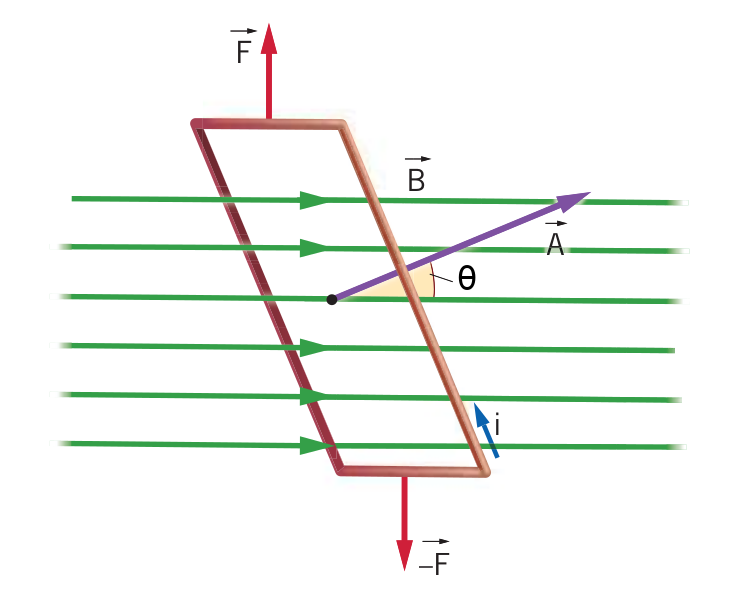
\includegraphics[width=.5\columnwidth]{img/momentomagnetico.png}
\end{figure}}
\end{frame}


\begin{frame}
\frametitle{Amperometro/galvanometro e voltmetro (1)}
\begin{figure}
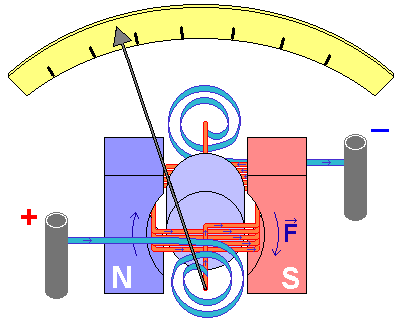
\includegraphics[width=.5\columnwidth]{img/galvanometro.png}
\end{figure}
L'amperometro va collegato \alert<1>{in serie} al circuito la cui corrente si vuole misurare.\pause

~

Possiamo anche realizzare un voltmetro (da collegare \alert<2>{in parallelo}).
\end{frame}

\begin{frame}
\frametitle{Amperometro e voltmetro (2)}
\begin{columns}
\begin{column}{0.4\textwidth}
\visible<1->{\begin{figure}
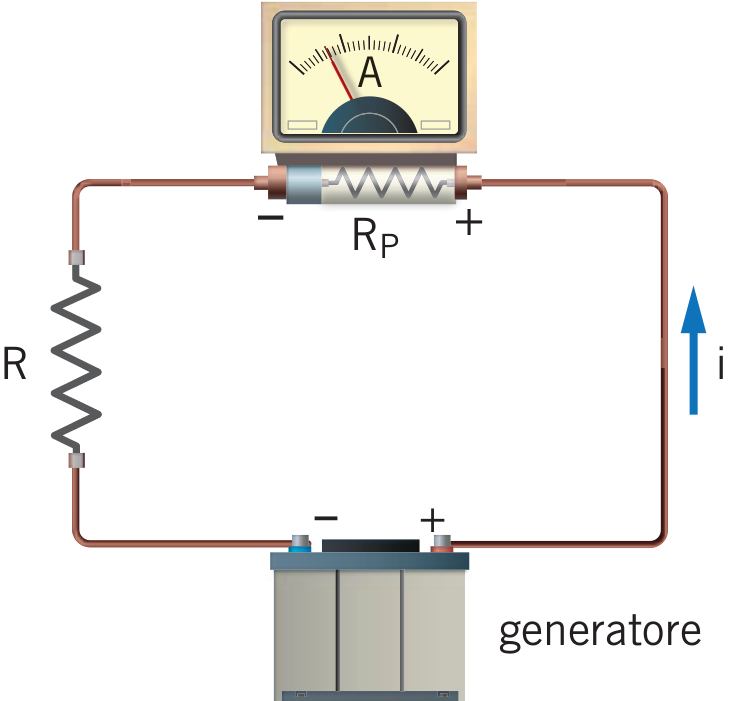
\includegraphics[width=\columnwidth]{img/amperometro.png}
\end{figure}}
\end{column}
\begin{column}{0.4\textwidth}
\visible<2->{\begin{figure}
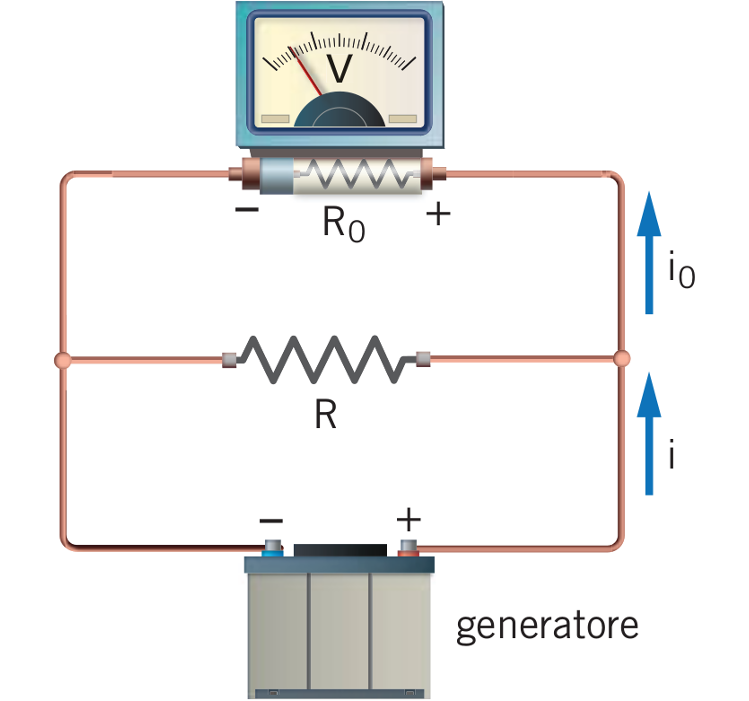
\includegraphics[width=\columnwidth]{img/voltmetro.png}
\end{figure}}
\end{column}
\end{columns}
\end{frame}



\section{Lorentz}

\begin{frame}
\frametitle{Forza magnetica senza filo}
Sappiamo:
\begin{itemize}
  \item da \O rsted, che \alert<1>{una corrente genera un campo magnetico};\pause
  \item da Faraday, che \alert<2>{una corrente subisce una forza magnetica}.\pause
\end{itemize}

~

È possibile verificare che :
\begin{itemize}
  \item \alert<3>{qualsiasi carica in moto genera un campo magnetico};\pause
  \item \alert<4>{qualsiasi carica in moto subisce una forza magnetica}.\pause
\end{itemize}

~

Ciò che vediamo accadere alle correnti (nei fili) è l'effetto macroscopico di tali fenomeni.
\end{frame}


\begin{frame}
\frametitle{Dimostrazione}
Ricordiamo:
\begin{center}
$ \vec{F} = i\vec{\ell}\times\vec{B} $\pause ~~~~~~~~~~~~~~ $ i = \dfrac{\Delta q}{\Delta t} $
\end{center}\pause

~

Immaginiamo una carica $ q $ che si muove, in un tempo $ \Delta t $, in un tratto di filo lungo $ \ell $.\pause
\begin{center}
$ \vec{F} = \dfrac{q}{\Delta t} \vec{\ell}\times\vec{B} =\pause q\left(\dfrac{\vec{\ell}}{\Delta t} \right)\times\vec{B} $ 
\end{center}\pause
Il termine tra parentesi è \alert<6>{$ \vec{v} $, la velocità della carica}.
\end{frame}


\begin{frame}
\frametitle{La forza di Lorentz}
\begin{block}{Forza di Lorentz}
Una carica $ q $, in moto con velocità $ \vec{v} $ in un campo $ \vec{B} $, subisce una forza:
\begin{center}
\colorbox{blue!30}{$ \vec{F} = q \vec{v} \times \vec{B} $}
\end{center}\pause
Il modulo della forza vale:
\begin{center}
$ F = qvB\sin\theta $
\end{center}
con $ \theta $ angolo tra i vettori $ \vec{v} $ e $ \vec{B} $.
\end{block}
\end{frame}



\begin{frame}
\frametitle{Regola della mano destra (attenzione!)}
\begin{columns}
\begin{column}{0.4\textwidth}
\visible<1->{\begin{figure}
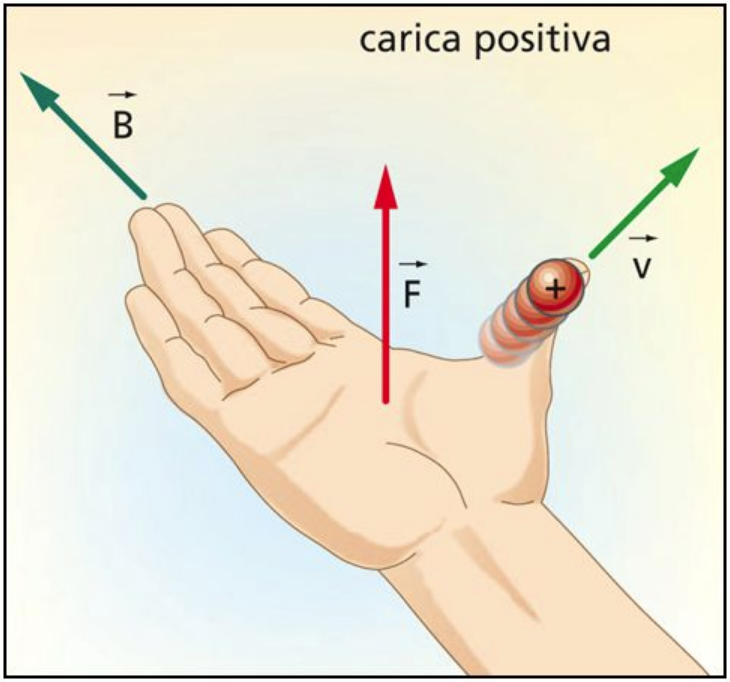
\includegraphics[width=\columnwidth]{img/lorentz1.png}
\end{figure}}
\end{column}
\begin{column}{0.4\textwidth}
\visible<2->{\begin{figure}
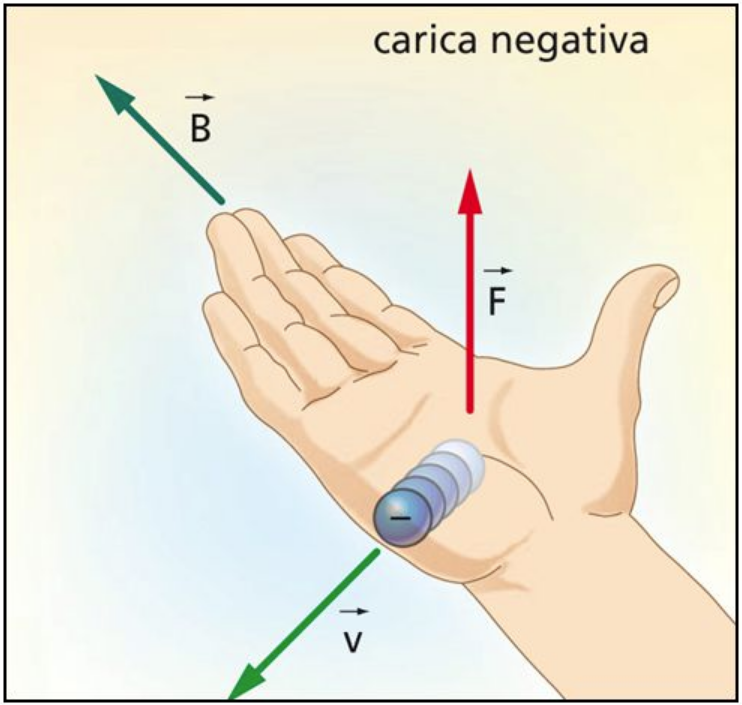
\includegraphics[width=\columnwidth]{img/lorentz2.png}
\end{figure}}
\end{column}
\end{columns}
\end{frame}

\begin{frame}
\frametitle{Esercizio}
\begin{exampleblock}{Moto di un protone}
  Un protone si muove in un campo magnetico uniforme di intensità $ 1,0 \times 10^{-2} \, T $, in una direzione perpendicolare a quella del campo magnetico. Sul protone agisce una forza di modulo $ 1,6 \times 10^{-16} \, N $.

  ~

  Calcola il modulo della velocità del protone.\hspace{\fill}[$ 1,0 \times 10^{5} \, \frac{m}{s} $]
\end{exampleblock} 
\end{frame}

\begin{frame}
\frametitle{Forza elettrica e magnetica su una carica}
Sappiamo che una carica $ q $:
\begin{itemize}
  \item subisce una forza elettrica $ F_e = qE $ se immersa in un campo elettrico $ \vec{E} $;\pause
  \item subisce una forza magnetica $ F_m = qvB $ se immersa in un campo magnetico $ \vec{B} $.
\end{itemize}\pause

~

Possiamo sfruttare queste due forze per costruire un \alert{selettore di velocità}.
\end{frame}


\begin{frame}
\frametitle{Selettore di velocità}
\begin{figure}
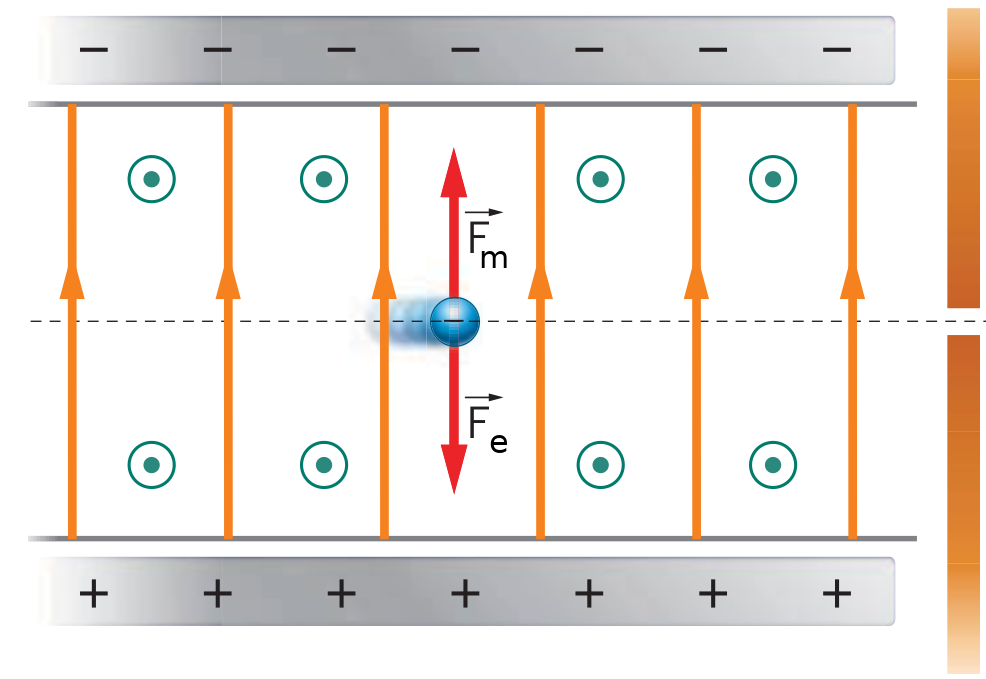
\includegraphics[width=.6\columnwidth]{img/selettore.png}
\end{figure}\pause
La carica prosegue di moto rettilineo sse:
\begin{center}
$ F_e = F_m ~~~ \pause\Longrightarrow ~~~ qE = qvB ~~~ \pause\Longrightarrow E = vB ~~~\pause\Longrightarrow$~~~\colorbox{blue!30}{$ v = \dfrac{E}{B} $} 
\end{center} 
\end{frame}


\begin{frame}
\frametitle{Lavoro della forza di Lorentz}
Ricordiamo che una forza $ \vec{F} $ che agisce su un corpo lungo uno spostamento $ \vec{s} $ esercita su di esso un lavoro:
\begin{center}
$ L = \vec{F} \cdot \vec{s} = Fs\cos\theta$ 
\end{center}
con $ \theta $ angolo tra $ \vec{F} $ e $ \vec{s} $.\pause

~

La fdL è perpendicolare al moto della carica ($ \theta = \frac{\pi}{2} $) e pertanto \alert<2->{la fdL non compie lavoro sulla carica su cui agisce}.\pause

~

Detto altrimenti:
\begin{itemize}
  \item la fdL non modifica l'energia cinetica $ K = \dfrac{1}{2}mv^2 $ della carica;\pause
  \item la fdL \alert<4->{modifica la direzione di $ \vec{v} $, non il suo modulo}.
\end{itemize}
\end{frame}

\begin{frame}
\frametitle{Forza centripeta}
Quando una forza agisce su un corpo, questo viene accelerato: 
\begin{center}
$ \vec{F} = m\vec{a} $
\end{center}\pause

~

Se la forza è perpendicolare alla velocità del corpo, essa agisce da forza centripeta e abbiamo un \alert<2>{moto circolare uniforme}.
\begin{center}
$ a_c = \dfrac{v^2}{r} ~~~~~~~\Longrightarrow~~~~~~~ F_c = m \dfrac{v^2}{r} $

~

\href{gif/centripeta.gif}{\beamergotobutton{GIF: Forza centripeta e moto circolare}}
\end{center}\pause

~

\alert<3>{La fdL, quando agisce su una carica, ne causa un moto circolare!}
\begin{center}
\href{video/Motomagnetico.mp4}{\beamergotobutton{Video: Moto di una carica in un campo magnetico}}
\end{center}
\end{frame}


\begin{frame}
\frametitle{Moto di una carica in un campo magnetico}
Calcoliamo il raggio dell'orbita (con $ \vec{v} \perp \vec{B} $):
\begin{center}
$ F_c = F_m $\pause

~

~

$ m\dfrac{v^2}{r} = qvB $\pause

~

~

$ \dfrac{mv}{r} = qB $\pause

~

~

\colorbox{blue!30}{$ r = \dfrac{mv}{qB} $}\pause
\end{center}
La misura di tale raggio è sfruttata dallo \alert{spettrometro di massa}.
\end{frame}


\begin{frame}
\frametitle{Esercizio}
\begin{exampleblock}{Moto circolare}
  Un elettrone che si muove alla velocità di $ 1,0 \times 10^{5} \, \frac{m}{s} $ entra in un campo magnetico perpendicolare alla direzione del moto. Si vuole che l'elettrone compia traiettorie circolari di raggio non superiore a $ 10 \, cm $.

  ~

  Come deve essere regolata l'intensità del campo magnetico?
  
  \hspace{\fill}[$ B \geq 5,7 \times 10^{-6} \, T $]
\end{exampleblock} 
\end{frame}

\begin{frame}
\frametitle{E se $ \theta \neq \dfrac{\pi}{2} $?}
\begin{figure}
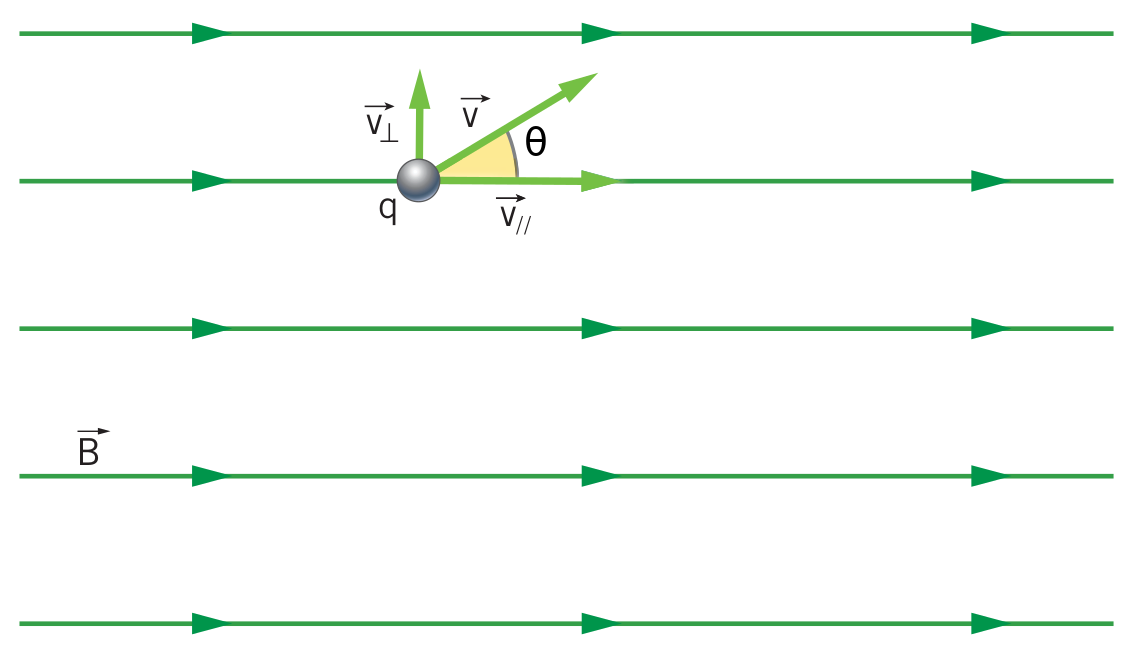
\includegraphics[width=.8\columnwidth]{img/elicoidale1.png}
\end{figure}
\end{frame}


\begin{frame}
\frametitle{Moto elicoidale}
Otteniamo un moto elicoidale a passo costante, composto da un moto circolare (in due dimensioni) e da uno rettilineo uniforme (nella terza).

~

\begin{figure}
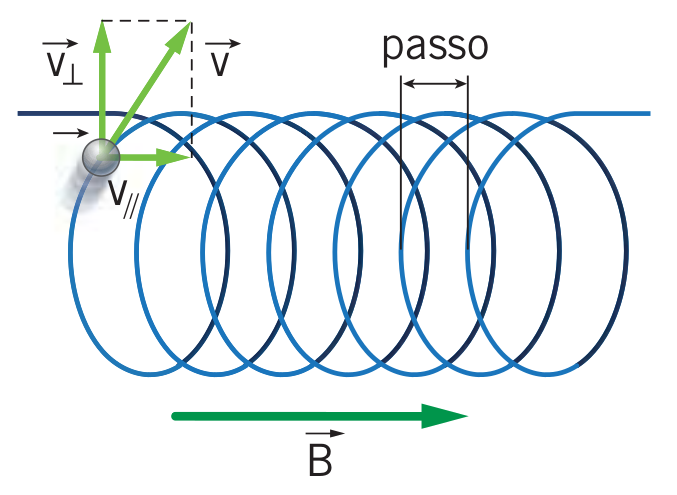
\includegraphics[width=.6\columnwidth]{img/elicoidale2.png}
\end{figure}
\end{frame}

\begin{frame}
\frametitle{Aurora boreale}
\begin{figure}
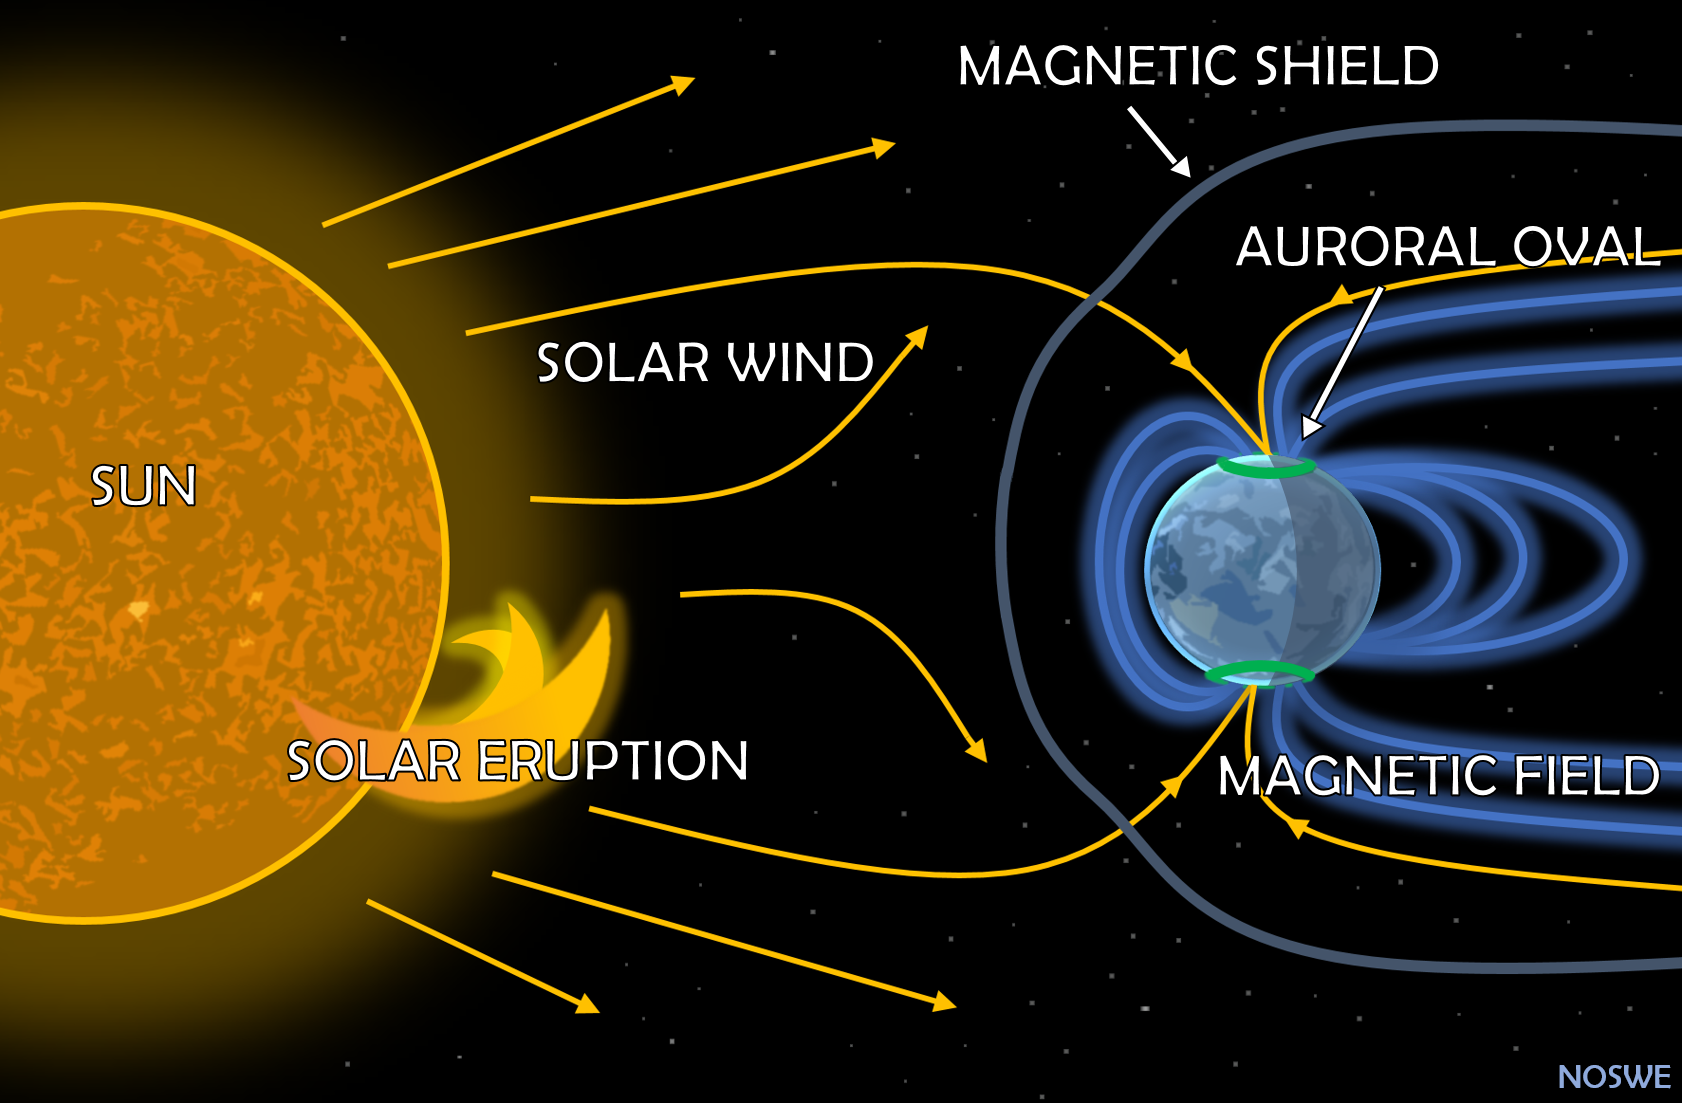
\includegraphics[width=\columnwidth]{img/ventosolare.png}
\end{figure}
\end{frame}


\section{Flusso e circuitazione}

\begin{frame}
\frametitle{Flusso  del campo magnetico}
Il flusso di $ \vec{B} $ attraverso una superficie $ S $ (eventualmente gaussiana) si definisce in modo analogo a quello di $ \vec{E} $. 
\begin{center}
\colorbox{blue!30}{$ \Phi_{S}(\vec{B}) = \vec{B} \cdot \vec{S} = BS\cos\theta $}
\end{center}\pause
Il flusso del campo magnetico si misura in \emph{weber}:
\begin{center}
$ [Wb] = [T\cdot m^2] $
\end{center}
\end{frame}


\begin{frame}
\frametitle{Il teorema di Gauss per il campo magnetico}
\begin{block}{Teorema di Gauss per il campo magnetico}
Il flusso del campo magnetico attraverso una superficie chiusa (gaussiana) è uguale a zero.
\begin{center}
\colorbox{blue!30}{$ \Phi_S (\vec{B}) = 0 $}
\end{center}
\end{block}\pause
Esistono cariche elettriche isolate, ma non monopòli magnetici (poli nord o sud isolati): \alert{per ogni linea di campo uscente ci sarà una linea di campo entrante}.
\end{frame}


\begin{frame}
\frametitle{Confronto tra i due teoremi di Gauss}
\begin{figure}
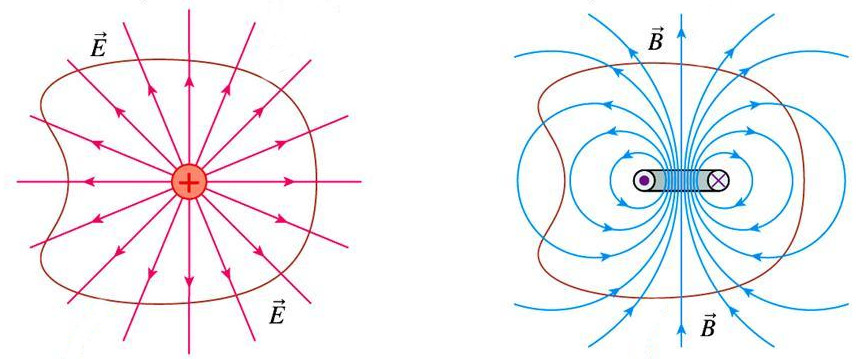
\includegraphics[width=\columnwidth]{img/confrontogauss.jpg}
\end{figure}
\end{frame}



\begin{frame}
\frametitle{Circuitazione del campo magnetico}
La circuitazione di $ \vec{B} $ lungo un cammino orientato $ \mathscr{L} $ si definisce in modo analogo a quella di $ \vec{E} $. 
\begin{center}
\colorbox{blue!30}{$ \Gamma_\mathscr{L} (\vec{B}) = \sum\limits_{i=1}^n \vec{B}_i \cdot \Delta \vec{\ell}_i =  \sum\limits_{i=1}^n B_i \Delta \ell_i \cos\theta_i $}
\end{center}
\end{frame}


\begin{frame}
\frametitle{Teorema di Ampère}
\begin{columns}
\begin{column}{0.5\textwidth}
Per $ \Gamma_B $ si dimostra che vale il \alert<1>{teorema di Ampère}, per cui:
\begin{center}
\colorbox{blue!30}{$ \Gamma_\mathscr{L} (\vec{B}) = \mu_0 \sum\limits_{k=1}^n i_k $}
\end{center}
dove $ i_k $ indica le $ k $ correnti concatenate a $ \mathscr{L} $.\pause
\end{column}
\begin{column}{0.4\textwidth}
\begin{figure}
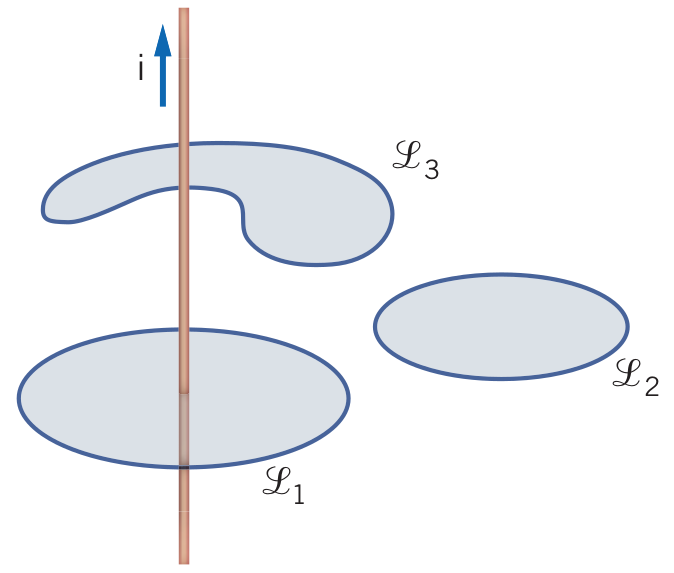
\includegraphics[width=\columnwidth]{img/teoremaampere.png}
\end{figure}
\end{column}
\end{columns}

~

~
   
Poiché il teorema di Ampère stabilisce che la circuitazione del campo magnetico può essere diversa da zero, affermiamo che, contrariamente al campo elettrostatico, \alert<2>{il campo magnetico non è conservativo}.
\end{frame}

\begin{frame}
\frametitle{Dimostrazione della legge di Biot-Savart}
\alert<1>{La legge di Biot-Savart}, che fornisce l'intensità del campo magnetico a distanza $ r $ da un filo percorso da corrente, \alert<1>{è un caso particolare del teorema di Ampère}.\pause

~

\begin{center}
$ \Gamma_\mathscr{L} (\vec{B}) = \sum\limits_{i=1}^n \vec{B}_i \cdot \Delta \vec{\ell}_i = \pause B \sum\limits_{i=1}^n \Delta \ell_i =\pause B 2 \pi r =\pause \mu_0 i $\pause
\end{center}
\begin{columns}
\begin{column}{0.4\textwidth}
da cui:
\begin{center}
\colorbox{blue!30}{$ B = \mu_0 \dfrac{i}{2\pi r} $}
\end{center}
\end{column}
\begin{column}{0.4\textwidth}
\begin{figure}
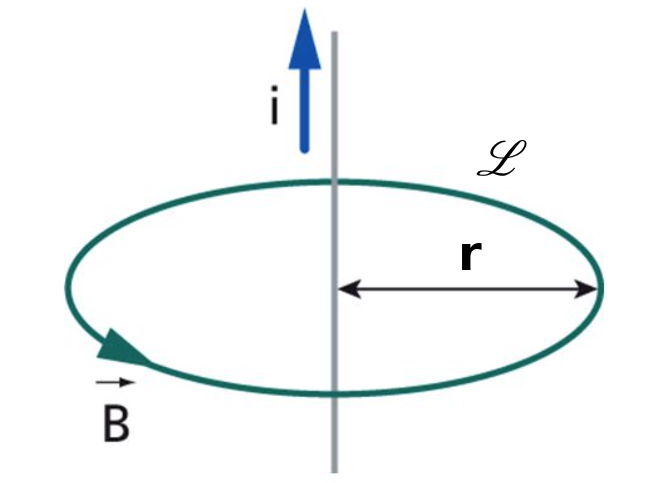
\includegraphics[width=\columnwidth]{img/biotsavart2.png}
\end{figure}
\end{column}
\end{columns}
\end{frame}




\section{Equazioni (1)}

\begin{frame}
\frametitle{Le equazioni di Maxwell (caso statico)}
  Riassumiamo quanto detto con le \alert{quattro equazioni di Maxwell} per il caso statico:\pause
\begin{enumerate}
  \item Teorema di Gauss per il campo elettrico
  \begin{center}
  \colorbox{blue!30}{$ \Phi_S (\vec{E}) = \dfrac{Q_{tot}}{\varepsilon_0} $}
  \end{center}\pause
  \item Teorema di Gauss per il campo magnetico
  \begin{center}
  \colorbox{blue!30}{$ \Phi_S (\vec{B}) = 0 $}
  \end{center}\pause
  \item Seconda legge di Kirchhoff (legge delle maglie)
  \begin{center}
\colorbox{blue!30}{  $ \Gamma_\mathscr{L} (\vec{E}) = 0 $}
  \end{center}\pause
  \item Teorema di Ampère
  \begin{center}
  \colorbox{blue!30}{$ \Gamma_\mathscr{L} (\vec{B}) = \mu_0 \sum\limits i_k $}
  \end{center}
\end{enumerate}
\end{frame}

\begin{frame}
  \frametitle{1.~Il teorema di Gauss per $ \vec{E} $}
    \begin{center}
  \colorbox{blue!30}{$ \Phi_S (\vec{E}) = \dfrac{Q_{tot}}{\varepsilon_0} $}
  \end{center}\pause
  Dice che:
  \begin{itemize}
    \item le linee del campo elettrico possono essere aperte;\pause
    \item esistono cariche elettriche isolate;\pause
    \item le cariche sono le sorgenti del campo elettrico.
  \end{itemize}
\end{frame}

\begin{frame}
  \frametitle{2.~Il teorema di Gauss per $ \vec{B} $}
    \begin{center}
  \colorbox{blue!30}{$ \Phi_S (\vec{B}) = 0 $}
  \end{center}\pause
  Dice che:
  \begin{itemize}
    \item per ogni linea di campo entrante c'è una linea di campo uscente, ovvero tutte le linee del campo magnetico sono chiuse;\pause
    \item non esistono poli magnetici isolati.
  \end{itemize}
\end{frame}

\begin{frame}
  \frametitle{3.~La seconda legge di Kirchhoff (legge delle maglie)}
  \begin{center}
\colorbox{blue!30}{  $ \Gamma_\mathscr{L} (\vec{E}) = 0 $}
  \end{center}\pause
  Dice che:
  \begin{itemize}
    \item il campo elettrostatico è conservativo.
  \end{itemize}
\end{frame}

\begin{frame}
  \frametitle{4.~Il teorema di Ampère}
  \begin{center}
\colorbox{blue!30}{$ \Gamma_\mathscr{L} (\vec{B}) = \mu_0 i_k $}
  \end{center}\pause
  Dice che:
  \begin{itemize}
    \item il campo magnetico non è conservativo;\pause
    \item le cariche in moto (le correnti) sono le sorgenti del campo magnetico.
  \end{itemize}
\end{frame}



\end{document}
